%****************************************************
%	CHAPTER 3 - Design Methodology
%****************************************************

\chapter{Design methodology}
\label{ch:ch3}
\section{Design overview}
\label{sec:ch3_design}

In Chapter \ref{ch:chapter2}, the critical areas, challenges and techniques used by remote sensing devices to meet the objectives outlined in \ref{sec:ch1.section1} were discussed.  Remote sensing devices aim to increase the temporal and spatial resolution of Southern Ocean data sets by increasing survivability and concentration of remote sensing platforms. The challenges identified in Chapter \ref{ch:chapter2} were the sea ice dynamics which can damage the device. Furthermore, strong wave activity and low temperatures which can freeze the device and degrade the battery life. A key difference between each device was the measurement objectives as shown in Table \ref{tab:device_deployment} which dictated the sensors, processing strategy and functionality of each system. \par

This section outlines the steps taken to identify the user requirements and translate them into hardware subsystems. The design phase began with a user requirements analysis. These requirements resulted in well-defined measurement objectives for the device and the selection of subsystems critical to the device functions. Then, a high-level system diagram was created to show the interaction of the subsystems within the system. This allowed for the selection of hardware components to satisfy the requirements for each subsystem. Finally, to ensure that the subsystems met the user requirements, a set of acceptance tests were derived. 


\section{User Requirements}
\label{sec:sec3_UR}

The user requirements analysis began with an identification of the project stakeholders shown in Appendix \ref{app:stakeholder}. Through constant engagement with the primary stakeholders, a set of user requirements was generated which identified the objectives the device would need to meet. The formatting, presentation and selection of these user requirements was done in accordance with IEEE Standards\footcite{IEEE_STD_UREQ}

\begin{table}[H]
    \centering
        \caption{User requirements obtained by meeting with the principal stakeholders. These will be used to determine the desired functionality of the buoy}
        \setlength{\extrarowheight}{5pt}
        \resizebox{\textwidth}{!}{%
    \begin{tabular}{ >{\centering\arraybackslash} m{0.3\textwidth}  >{\raggedright\arraybackslash} m{0.7\textwidth} }
    \hline
       \textbf{User Requirement ID}  & \textbf{Description}  \\
       \hline
       \hline
       UR001  & System must be able to withstand the Southern Ocean climate.\\
       \hline
       UR002 & System must be able to transmit data remotely without additional infrastructure or user input. \\
       \hline
       UR003 & System shall provide higher temporal and spatial resolution data. \\
       \hline
       UR004 & System must be capable of measuring  ice floe dynamics and environmental conditions surrounding sea ice formation. \\
       \hline
       UR005 & System must be user-friendly and easy to deploy.\\
       \hline
       UR006 & System Must be cost effective. \\
       \hline
       UR007 & System must be able to store and process data in an organised manner. \\
       \hline
    \end{tabular}}

    \label{tab:user_reqs}
\end{table}

\subsection{Analysis of UR001}
\textit{System must be able to withstand the Southern Ocean climate.}

\textcite{kohout2015device} encountered 7 m swell and 25 $\text{ms}^{-1}$ winds during their deployment in the marginal ice zone which lead to the immediate failure of one of their systems \cite{kohout2015device}. Strong wind and waves were also observed by \textcite{vichi2019effects,alberello2019drift} during their deployment which has been attributed to multiple cyclonic events coinciding with the deployment of the WIIOS buoys. The effects of wind and waves result in the delay of consolidation of sea ice at the edge of the marginal ice zone  which created survivability challenges for the devices. Additionally, \textcite{albarello2020drift} showed that wind speed resulted in ice floe drifting at $0.35$ $\text{ms}^{-1}$. Placing the buoy close to the surface of the ice subjects it to collisions, breaking and rafting which resulted in the failures of \cite{doble2017robust,rabault2019open}. Snow and ice formation on the surface of the floe can bury the device \cite{doble2017robust}  and constant wave energy on unconsolidated ice cause flooding which can further damage the devices. A device that is elevated above the surface while tethered to the floe can reduce exposure to these events however the buoy elevation must be at least 1 m to compensate for snow growth \cite{barber2005microwave}. \par

Furthermore, for a device to survive in the Southern Ocean, the software must contain a robust set of error checking for each module. The software should ensure that critical subsystems are functional and responsive while constantly providing feedback on statuses. Should a module be damaged or go offline, the software should flag this issue, identify the failure and attempt to rectify it. Alternatively, if the failure is critical, the device should flag the module as malfunctioning and continue to operate without it.

\subsection{Analysis of UR002}
\textit{System must be able to transmit data remotely without additional infrastructure or user input.}

\textcite{kennicutt2016delivering} shows a fundamental lack of infrastructure on the Antarctic continent including data networks. Operations taking place on sea ice are isolated from any resources that exist via Antarctic bases. Sea ice in the marginal ice zone is subject to conditions inhospitable to humans \cite{kennicutt2016delivering}. Therefore access to the buoys is limited once the device is deployed often making it difficult to retrieve. The life cycle of sea ice presents an additional access challenge through the consolidation of sea ice  during the freezing periods and melting  of the ice floes during the warming periods \cite{womack_2020}. Additionally, manned expeditions are typically inflexible \cite{kennicutt2016delivering} resulting in additional challenges in retrieving the buoy and hence the data. Therefore, most devices deployed in the region are designed to be expendable (\cite{kohout2015device,rabault2019open,trident}). These device circumvent this by using satellite networks with global coverage such as Iridium\footnote{See Chapter \ref{ch2:secdevice}} which allows the users to receive data and status updates from the buoy without needing to retrieve the devices. 

The lack of user input implies that device routines and sub routines must be performed automatically. The device should control and sample sensors in a fixed, predictable manner ensuring that the correct data is sampled during the correct periods. Furthermore, the device needs to transmit data over the Iridium network. Therefore the software is required to control the interactions with the mode ensuring that it is functional. The software should condense data to fit the bandwidth of the device and ensure it is successfully uploaded to the transmission buffer. Finally, the software should be able to check for sufficient network availability and initiate a transmission. Should an error occur, the software needs to respond and handle it efficiently.

\subsection{Analysis of UR003}
\textit{System shall provide higher temporal and spatial resolution data.}

Phases of the sea ice life cycle are defined by periods of freezing followed by periods of melting \cite{barber2005microwave} with maximum extents occurring in winter (freezing) and summer (melting) respectively \cite{barber2005microwave}. The formation and consolidation of sea ice floes are influenced by atmospheric and oceanic processes resulting in the delay of sea ice consolidation \cite{vichi2019effects,albarello2020drift}. Each period coincides with a seasonal cycle typical lasting a few months \cite{vichi2019effects,alberello2019drift,barber1948generation} which is the length of time a buoy needs to survive to provide sufficient data on a temporal scale. \par 

Increasing remote sensing in the region is also required to provide spatial coverage \cite{albarello2020drift}. Certain observational methods such as satellite observation are performed on a 10 m scale \cite{galin2011validation} where sea ice variability can scale down to the cm \cite{vichi2019effects}. \textcite{doble2017robust} achieved large spatial coverage by deploying the devices in clusters of five every 5 km. Additional deployments from \cite{vichi2019effects}, \cite{kohout2015device} and \cite{albarello2020drift}
also achieved this by deploying multiple systems spaced 3 to 4 m apart \cite{vichi2019effects}. Therefore increasing the spatial resolution can be achieved by increasing the concentration of devices in an area spaced apart. \par 

For a remote sensing device to survive the required period, a built-in power source is required to maintain functionality without constant maintenance. This power supply primarily needs to come from a replenishable source. \textcite{doble2017robust} and \textcite{rabault2019open} coupled battery arrays to a rechargeable power system which showed promise however, insufficient cloud cover \cite{doble2017robust} resulted in the solar panel being underutilised. As discussed in Chapter \ref{ch2}, commercial batteries are readily available and well-specified to supply power for long periods \cite{rabault2017measurements}. However, the system must conserve energy. Otherwise, this could result in low survival rates \cite{kohout2015device}. Additionally, batteries in sub-zero temperatures have a significantly reduced capacity of up to 50\% \cite{doble2017robust}.

Therefore, the software needs to contain power monitoring capabilities. A sensor should monitor the current and power usage of the device and provide feedback to the system. The device software should be optimized to conserve power which means turning off sensors that are not in use and entering low power mode during periods of inactivity. Finally, the software needs to handle power events that could disrupt the functionality of the buoy such as brownouts and power resets. The software should be able to recognize when the power is too low to operate and respond accordingly.

\subsection{Analysis of UR004}

\textit{System must be capable of measuring ice floe dynamics and environmental conditions surrounding sea ice formation.}

As discussed in Chapter \ref{ch2:secdevice}, in situ, remote sensing devices have been deployed in the Southern Ocean with specific measurement objectives. Table \ref{tab:device_deployment} shows that the following measurements were common to one or more devices:
\begin{itemize}
	\item Ice drift
	\item Collisions between ice floes
	\item Waves in ice
	\item Ambient temperature
	\item Atmospheric pressure
\end{itemize}

\subsubsection{Meteorological sensing requirements}

Temporal resolutions and measurement standards need to be taken in accordance with the World Meteorological Organisation to ensure effective communication and standardisation of the data sets \cite{worldmeteorologicalorganization_2010}. For environmental data and wave spectra, the data are provided in Table \ref{tab:metocean} below:

\begin{table}[H]
	\centering
	\caption{Comparison of standard measurements for meteorological data including temporal resolution, measurement unit and accuracy from: \cite{worldmeteorologicalorganization_2010}}
	\setlength{\extrarowheight}{5pt}
	\begin{tabular}{lll}
		\hline
		\textbf{Variable Name}  & \textbf{Resolution} & \textbf{Accuracy}\\
		\hline
		\hline
		Temperature & 1 hour & $\pm$0.5 K \\
		
		Pressure & 1 hour & $\pm$ 0.5 HPa \\
		
		Wind Speed & 1 hour & $\pm \text{2 ms}^{-1}$\\
		\hline
	\end{tabular}
	\label{tab:metocean}
\end{table}

Meteorological data should be sampled from a height of 1 to 40 m  \cite{worldmeteorologicalorganization_2010}. Therefore, all meteorological sensors should be mounted 1 m above the ground to meet these standards. Additionally, the software should be capable of retrieving data from a temperature and pressure sensor. The software should also contain error checking to ensure robust sampling and reliable data from the sensors. \par 

\subsubsection{Ice drift sensing requirements}

\textcite{trident,uptempo,kohout2015device} and \textcite{albarello2020drift} show that ice drift measurements can be taken using a GNSS tracker can be used to monitor by recording the global coordinates against an accurate time reference. \textcite{alberello2019drift} show that temporal resolutions affect the behaviour of drift data. Devices that went into low power mode during deployment (\cite{vichi2019effects,alberello2019drift}) had decreased sampling rates which failed to capture ice drift oscillations. \textcite{albarello2020drift} further show that a temporal resolution of 3 hours is required to capture ice drift oscillations. Additionally, the GPS reading can be affected by the number of satellites picked up by the receiver (dependent on the receiver antenna gain) \cite{spilker1996global}, the spread of satellites and the angle of elevation above the horizon. A characteristic of this error is called the dilution of precision (DOP). This value details the positional or temporal measurement inaccuracy. Moreover, the software needs to accommodate a GPS module and interface with it through a suitable communication port. The software needs to sample the GPS at a frequency of once every 3 hours or less. Finally, the software should configure the GPS module to transmit diagnostic information, positional error and temporal error information in addition to time and date information.\par 

\subsubsection{Waves in ice sensing requirements}

Wave in ice measurements play a critical role in understanding the formation of sea ice in the marginal ice zone \cite{alberello2019drift}. Low frequency, high energy waves propagate through the area and displace the ice floes \cite{womack_2020}. Current devices such as those developed by \cite{rabault2017measurements,thomson2012wave,kohout2015device} utilise either a statistical \cite{kuik1988method} or spectral \cite{earle1996nondirectional,welch1967use} approach which allows for measurements of waves independent of the dynamics of the ice floe. These methods require roll, heave, pitch and vertical acceleration measurements for 1000 s at sample rates above 0.5 Hz, which corresponds to the upper band of ocean waves \cite{earle1996nondirectional}. The software should be capable of interfacing with an IMU and should ensure that data is sampled at a fixed sample rate for the required period. The software should also store the data in an area with sufficient space. Finally, the software should contain error checking algorithms to ensure robust communication with this device. \par 

\subsection{Analysis of UR005}

\textit{System must be  user-friendly and easy to deploy}

Table \ref{tab:device_price} shows the weight of each system. Notably, the lightest device being the Trident buoy at 0.42 kg and the heaviest being the buoys by \textcite{doble2017robust}. The weight of the device significantly affects the deployment protocol. Heavy devices will require a large team to deploy the device and specialised courier methods to transport it such as those described in \textcite{doble2017robust}. Devices that weighed 4.5 kg to 30 kg were light enough to be carried by one person and deployed much faster.

The deployment is also affected by the set up of the device. The SIMB Buoy, while being relative light, requires a team to assemble the components on the ice and drill a hole to place it in \cite{PLANCK2019102792}. \textcite{kennicutt2016delivering} shows that certain polar regions are too dangerous for manned missions, which can limit the deployment location and time frame the crew can spend setting up the buoy. However, systems that are relatively easy to deploy (Trident, WIIOS, SWIFT) allow for sensing near dangerous environments such as the ice edge of the marginal ice zone. These devices are preassembled and set up leading to a "drop and go" style deployment from ship cranes \cite{vichi2019effects,alberello2019drift} or boats \cite{rabault2019open,kohout2015device}. The software should be configured to begin execution as soon as the device is operational. Software settings and parameters should be loaded into permanent storage and the sensors should be calibrated before being sent on the expeditions.

\subsection{Analysis of UR006}

\textit{System must be cost effective}

\textcite{PLANCK2019102792,guimaraes2018surface,rabault2019open} consider cost to be a significant constraint in designing a system. Additionally, some devices such as SIMB buoy, gradually factored in price after two iterations \cite{planck2019evolution}. This shows that optimising device performance for cost is critical for increasing the affordability and availability of devices. An affordable system Table \ref{tab:device_price} showed a comparison of reported costs and wughts for each system where applicable.
 
from Table \ref{tab:device_price} we can see from the cost breakdown that \textcite{rabault2019open} succeeded in creating a low cost buoy through the use of open source hardware and off-the-shelf components resulting in this device having the lowest reported price out of all the system. The next cheapest device is the Trident buoy which is only R300.00 more expensive than the WIIB. However, this device contains fewer sensors and is only capable sea ice drift and temperature measurements. On average, commercial systems (UptempO, Polar ISVP, Trident) proved to be significantly more expensive than research devices with similar attributes. However, due to the absence of prices for SWIFT, WIIOS and Trident it is difficult to draw conclusions from this comparison. Furthermore, commercial systems had design capabilities to design and print custom circuit boards and chip sets while research systems (SWIFT, WIIB, WIIOS) did not have such capabilities. Therefore, the developers optimised for procurement time by using off the shelf components \cite{kohout2015device,rabault2019open}. A novel sensing device that is cost optimized should result in an overall cost cheaper than the devices in table \ref{tab:device_price} with comparable performance, this will also allow for quicker and cheaper device procurement allowing for more devices to be produced for deployment thereby allowing for a larger spatial area in the marginal ice zone to be covered.

\subsection{Analysis of UR007}

\textit{System must be able to store and process data in an organised manner}

The proposed system will require multiple subsystems to satisfy the user requirement UR004. These subsystems will generate large volumes of data that needs to be stored and organised efficiently. As shown in the discussions for user requirements UR001 to UR005, the system will require multiple sensors and modules. Each module has different operational and communication requirements. Therefore, a suitable processor needs to be selected to provide sufficient ports to interface with each sensor. This processor should accommodate sufficiently high volumes of data with a wide enough byte size to accept sensor data without calculation errors. The software will need to meet the requirements of each sensor and sequence these functions into a routine. This can be achieved by developing sensor libraries for each device. Included in these libraries will be initialisation routines, peripheral communication drivers and sensor sampling routines to meet the requirements for each sensor. Furthermore, as shown in the discussion above, each sensing activity is time-critical. This places a strict timing requirement on the device to ensure the integrity of the data set on a temporal scale. Therefore, an accurate timing reference is required in the form of a real-time clock (RTC). \par 

Additionally, Each sensor has a different data rate requirement. Some sensors will need to stream large volumes of data of an unknown length. To deal with this, efficient data acquisition techniques need to be implemented by the software to accommodate these volumes. Such techniques include setting up direct memory access (DMA) channel in a circular buffer to stream data to a memory location with an input capture timer on slave reset mode to close the channel when the data stream is completed.\par 

Finally, long periods of inactivity between measurements can result in wasted power. The discussion of user requirement UR003 showed that the software should turn the device off or into low power mode during these periods. If the data is in the processor memory when the device is off, it could get lost. Therefore, a permanent storage device is required to store data during these periods of inactivity. The software should include functions to read from the storage space and write to it efficiently. Additional error checks should be written to ensure the storage device is online, operational and the data has not been corrupted.

Finally, the aforementioned hardware and software modules need to be verified with a suite of acceptance tests to ensure that all the user requirements have been met. 


\section{Functional requirements}
\label{sec:ch3_FR}
Analysis of the aforementioned user requirements resulted in the procurement of a set of functional requirements that dictate how the buoy will function.

\subsection{Operational requirements }

\begin{table}[H]
    \centering
    \caption{Requirements addressing the mechanical needs for the system during operation.}
    \setlength{\extrarowheight}{5pt}
    \resizebox{\textwidth}{!}{%
    \begin{tabular}{>{\centering\arraybackslash}m{0.2\textwidth}>{\RaggedRight}m{0.7\textwidth} >{\RaggedRight}m{0.25\textwidth}}
    \hline
         \textbf{Requirement ID} & \textbf{Description} & \textbf{User requirements addressed}\\
         \hline
         \hline
         \multirow{2}{0.2\textwidth}{FR001} & \multirow{2}{0.7\textwidth}{The System shall have a protective enclosure against precipitation and frost.} & UR001\\ &&UR005 \\
         \hline
         \multirow{2}{0.2\textwidth}{FR002} & \multirow{2}{0.7\textwidth}{The enclosure shall be constructed from strong, corrosion resistant materials with strong thermal characteristics.} &  UR001 \\ && UR005 \\
         \hline
         \multirow{1}{0.2\textwidth}{FR003}& The device will protect electronics from internal humidity. & UR001\\
         \hline 
          \multirow{2}{0.2\textwidth}{FR004}& \multirow{2}{0.7\textwidth}{The electronics will be elevated above the ground by 1 m.} & UR001\\ &&UR005 \\
         \hline
         \multirow{2}{0.2\textwidth}{FR005} & \multirow{2}{0.7\textwidth}{All subsystems shall be rated for extreme temperatures.} & UR001\\ && UR003\\
         \hline
         \hline
    \end{tabular}}

    \label{tab:hard_funcreqsl}
\end{table}

\subsection{Electronic requirements}

\begin{table}[H]
    \centering
    \caption{Requirements addressing the electronic needs for the system including the modules, components and sensors that satisfy the user requirements.}
    \setlength{\extrarowheight}{5pt}
    \resizebox{\textwidth}{!}{%
    \begin{tabular}{>{\centering}m{0.2\textwidth}>{\RaggedRight}m{0.7\textwidth} >{\RaggedRight}m{0.25\textwidth} }
    \hline
         \textbf{Requirement ID} & \textbf{Description} & \textbf{User requirements addressed}\\
         \hline
         \hline
         \multirow{1}{0.2\textwidth}{FR006} & System will transmit data via Iridium satellite network. & UR002\\
         \hline
         \multirow{2}{0.2\textwidth}{FR007} & \multirow{2}{0.7\textwidth}{Device shall be battery powered.} & UR001 \\ && UR003\\
         \hline
         \multirow{1}{0.2\textwidth}{FR008} & System shall measure ice drift using a  global positioning system (GPS). & UR004\\
         \hline
          \multirow{1}{0.2\textwidth}{FR009}& Device shall measure ambient temperature. & UR004\\
         \hline
         \multirow{1}{0.2\textwidth}{FR010} & Device shall measure atmospheric pressure & UR004 \\
         \hline
        \multirow{1}{0.2\textwidth}{FR011}  & Device shall contain an inertial measurement unit (IMU) to record acceleration (3-axes) and rotation (3-axes) of an ice floe. & UR004 \\
         \hline
         \hline
    \end{tabular}}
    \label{tab:other_funcreqs}
\end{table}

\subsection{Software requirements}

\begin{table}[H]
    \centering
    \caption{Software functional requirements for the system addressing the system function, performance, operation and control during the lifetime of the device.}
        \setlength{\extrarowheight}{5pt}
    \resizebox{\textwidth}{!}{%
    \begin{tabular}{>{\centering}m{0.2\textwidth}>{\RaggedRight}m{0.7\textwidth} >{\RaggedRight}m{0.25\textwidth} }
    \hline
        \textbf{Requirement ID} & \textbf{Description} & \textbf{User requirements addressed}\\
         \hline
         \hline
        \multirow{2}{0.2\textwidth}{FR012} &  \multirow{2}{0.7\textwidth}{Device to contain sufficient memory for data storage.} & UR006\\ && UR007 \\
         \hline
        \multirow{2}{0.2\textwidth}{FR013} &  \multirow{2}{0.7\textwidth}{Device to contain a processing unit to control sensors and process data.} & UR006\\ && UR007\\
         \hline
         \multirow{3}{0.2\textwidth}{FR014} &  \multirow{3}{0.7\textwidth}{Device to be optimised for low-power consumption and power event handling.} & UR003\\&& UR006 \\&& UR007  \\
         \hline
         \hline
    \end{tabular}}
    \label{tab: soft_funcreqsl}
\end{table}

\subsection{Other requirements}
\begin{table}[H]
    \centering
    \caption{ Other system requirements being addressed.}
   \setlength{\extrarowheight}{5pt}
\resizebox{\textwidth}{!}{%
	\begin{tabular}{>{\centering}m{0.2\textwidth}>{\RaggedRight}m{0.7\textwidth} >{\RaggedRight}m{0.25\textwidth} }
		\hline
		\textbf{Requirement ID} & \textbf{Description} & \textbf{User requirements addressed}\\
    \hline
    \hline
   \multirow{1}{0.2\textwidth}{FR015} & Device shall be calibrated prior to shipping and delivered in a state where it can be deployed at a moment's notice & UR005 \\
    \hline
   \multirow{1}{0.2\textwidth}{FR016} & The Device will cost less than currently available systems. & UR006 \\
    \hline
    \hline
    \end{tabular}}
    \label{tab:elec_funcreqs}
\end{table}

\section{System overview}
\label{sec:ch3_sysoverview}
To meet the functional requirements, the overall system was designed using a top down approach. The requirements highlighted in Tables \ref{tab:hard_funcreqsl} to \ref{tab:other_funcreqs} will be used to identify key subsystems to achieve the required functionality.

\begin{table}[H]
    \centering
    \caption{Table showing the subsystems that are critical to the functionality of the buoy and the level of importance indicated by rank}
    \setlength{\extrarowheight}{2.5pt}
    \begin{tabular}{l c }
    \hline
    \textbf{Name}  & \textbf{Rank}\\
    \hline
    \hline
    Firmware & 1\\
    \hline
    Power system & 2 \\
    \hline
    Communication module  & 3\\
    \hline
    Processor & 4\\
    \hline
    Sensors & 5\\
    \hline
    Permanent storage  & 6 \\
    \hline
    Mechanical features & 7 \\
    \hline
    \hline
    \end{tabular}

    \label{tab:subsys}
\end{table}

The firmware is the most critical subsystem in the device and ranks the highest in terms of priority. The firmware is crucial for the operation of the device and to control all the modules. The next most critical component is the power system. Any failures in the power system will cause the device to stop functioning.  All device components need to be rated for subzero operation to ensure robust operation. A voltage regulator will be included to ensure a constant voltage. Finally, a power sensor will be included to monitor the batteries and warn the system when the batteries are almost depleted. \par 

After the power system is the communication subsystem as Iridium will be used to transmit the data obtained by the system. Should this device fail, the device will be unable to transmit data unless it is retrieved. Satellite communication for Iridium is performed using a satellite mode while GPS communication is performed using a GPS receiver. They require, clear, unobstructed views of the satellites which can be achieved with high-gain antennas. These devices need to mounted as close to the sky as possible.\par

The sensors are the primary interface between the system and the environment. The electronics need to be as close to the exterior of the system as possible to measure ambient temperature and pressure. The IMU can be mounted anywhere inside the buoy however, the device needs to be calibrated for its position on the buoy as well as its orientation inside. \par

The sensors will interface with a central processing system which will control the sensors and sample data from them. Data coming from the sensor will be processed and stored in packets in a permanent memory storage system. Finally, a metal stand will be created to anchor the device to an ice floe and suspend the electronics well above the sea ice surface to prevent it from being covered in snow. The electronics will be placed in a thermal-resistant and waterproof enclosure to protect the system with desiccant placed inside to prevent moisture from interfering with the device. A block diagram of the proposed system is shown in the figure below.

\begin{figure}[H]
    \centering
    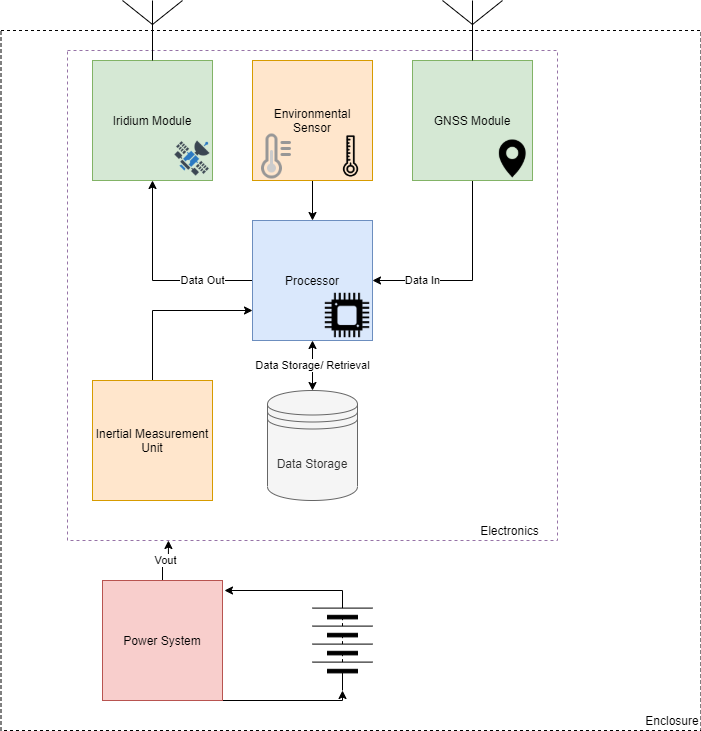
\includegraphics[width=\linewidth]{SHARC_NODE}
    \caption{Block diagram of the proposed autonomous system showing subsystem arrangement, data flow and interfaces with the environment.}
    \label{mbuoy}
\end{figure}

These subsystems can be further broken down into components requirements as shown in the figure below

\begin{figure}[H]
    \centering
    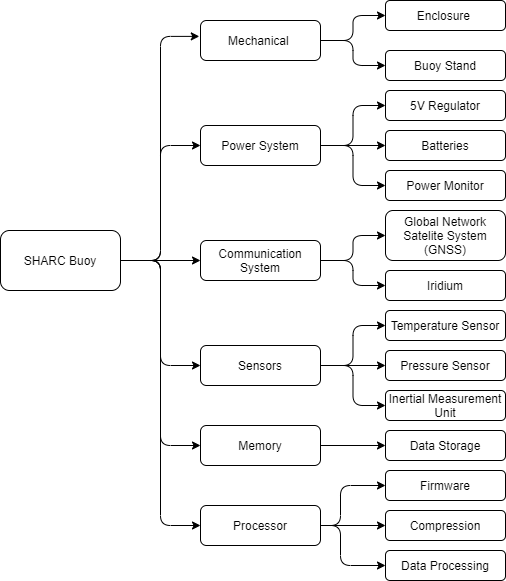
\includegraphics[width=0.8\textwidth]{Subsystem_Diagram.png}
    \caption{Breakdown of subsystems from table \ref{tab:subsys} into usable components.}
    \label{fig:ss_breakdown}
\end{figure}



\subsection{Technical specifications}

These technical specifications will be used to determine what hardware is required to construct the subsystems as showing in Figure \ref{mbuoy} above.

%%%FIX THIS TABLE

\begin{table}[H]
    \centering
    \caption{Technical specifications for the overall system}
     \setlength{\extrarowheight}{5pt}
    \resizebox{\textwidth}{!}{%
    \begin{tabular}{>{\centering\arraybackslash}m{0.25\textwidth}>{\raggedright\arraybackslash}m{0.6\textwidth} >{\raggedright\arraybackslash}m{0.35\textwidth} }
        \hline
         \textbf{Specification ID} & \textbf{Description} & \textbf{Functional requirement addressed} \\
         \hline
         \hline
         \multirow{2}{0.2\textwidth}{SP001} & \multirow{2}{0.6\textwidth}{Enclosure built using thermal resistant plastic.} & FR001\\ && FR002\\
         \hline
         \multirow{3}{0.2\textwidth}{SP002}  & \multirow{3}{0.6\textwidth}{Electronics to be mounted on a 1.5 m stand constructed from non-corrosive metal.} & FR002\\ && FR003\\ &&FR004\\
         \hline
         \multirow{1}{0.2\textwidth}{SP003} & System to include desiccant packets inside the enclosure. & FR003 \\
         \hline
         \multirow{1}{0.2\textwidth}{SP004} & Device to have a temperature operating range of $-40 ^\circ \text{ C to } 20 ^\circ$ C with $ 1^\circ$ C uncertainty. & FR009 \\
          \hline
         \multirow{1}{0.2\textwidth}{SP005}& Subsystems to be rated for $3.3 \textbf{ V to } 5$ V power. & FR008 \\
          \hline
         \multirow{1}{0.2\textwidth}{SP006}& Device shall survive for 1 month on a single set of cells & FR007 \\
          \hline
         \multirow{1}{0.2\textwidth}{SP007} & The device should cost less than R10,000 & FR016 \\
         \hline
         \multirow{1}{0.2\textwidth}{SP008} & System will contain flash chips for permanent storage. & FR012 \\
         \hline
         \multirow{1}{0.2\textwidth}{SP009}& System will use the STMicroelectronics STM32 series of microcontroller. & FR013 \\
         \hline 
         \multirow{1}{0.2\textwidth}{SP010} & The system shall be supplied by a regulated 5 V supply.  & FR014 \\
         \hline
         \multirow{1}{0.2\textwidth}{SP011} & The low power threshold occurs for voltages < 5 V & FR014 \\
         \hline 
         \multirow{4}{0.2\textwidth}{SP012}& Maximum current operations: & \multirow{4}{0.2\textwidth}{FR0014}\\
            &500 mA maximum start-up current. & \\
            &100 mA maximum active current. & \\
            &10 mA sleep current.& \\
         \hline
         \multirow{1}{0.2\textwidth}{SP013} & Device to be powered off or placed in sleep mode when inactive. & FR014 \\
         \hline
         \hline
    \end{tabular}}

    \label{tab:sys_specs}
\end{table}
\subsection{Acceptance test protocols}

In this section, the acceptance testing protocols for hardware and software modules is provided. These tests are designed to ensure that the devices meet the functional requirements outlined in table \ref{tab:hard_funcreqsl} to \ref{tab:elec_funcreqs}. A full description of the acceptance test protocols can be found in Appendix \ref{app:atp}. The goal of the acceptance criteria of each test as well as the the targeted module is given in table x below.

\begin{table}[H]
	\caption{A summary of acceptance test protocols from Appendix \ref{app:atp} showing the target and purpose of the test.}
	\label{tab:acceptance_test_summary}
	 \setlength{\extrarowheight}{5pt}
	\resizebox{\textwidth}{!}{%
		\begin{tabular}{cll}
			\hline
			\textbf{Acceptance test} & \textbf{Target} & \textbf{Purpose}\\
			\hline
			\hline
			AT001 	& Sensor modules. & Ensure module is online and functional \\
			\hline
			AT002	& All hardware modules.  & Test for faults and errors. \\
			\hline
			AT003 	& Device components. & Ensure selected components are rated for this application.\\
			\hline
			AT004	& Sensor peripheral libraries. & Verify software correctly interfaces with subsystem modules. \\
			\hline
			AT005	& Full system. & Ensuring an accelerated functional cycle meets the timing and sensing requirements. \\
			\hline
			AT006	& Sensor modules. & Calibrate the sensors against a known reference. \\
			\hline
			AT007	& Power subsystem. & Verify the power system meets the user requirements. \\
			\hline
			AT008	& Full system. & Ensure the device can operate in low temperatures. \\
			\hline
			AT009	&  Full system. & Ensure device functions in a remote environment. \\
			\hline
			\hline
		\end{tabular}
	}
\end{table}

%TODO create a summary of atp protocols as discussed with robyn

\section{Conclusion}

To summarise, this chapter outlines the design procedure for identifying critical subsystems and technical specifications to meet the user requirements. This will provide the basis for component and module selection which will be discussed in the next chapter.

\chapter{Platform design}
\label{sec:ch3_platform}

\section{Mechanical Features}

The mechanical design for the system falls outside the scope of this project however, it forms an integral part in protecting the electronics. The principle goal of the mechanically features are to anchor the device to the ice floe and protect it from the harsh environment. A buoy stand was designed by Keith Hutchinson with the University of Cape Town Workshop to satisfy this requirement. The stand is 1.2m tall with a base cross section of 0.71m and contains a cylindrical housing at the top where the device will be placed. A screw hole in the side of the stand allows the buoy to be fast-end to the stand to prevent it from falling out. The base of the stand is pyramid shaped with metal spikes to anchor the system to an ice floe. Due to the height of the stand, the system may be susceptible to tipping. This has been overcome by constructing the base to be heavier than the top thereby lowering the center of gravity. The stand was originally designed for the Trident buoys and this design has been modified by increasing the radius of the housing. 

\begin{figure}[H]
    \centering
    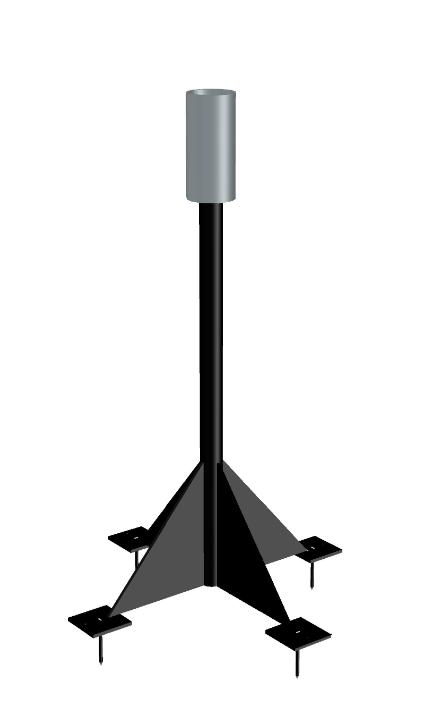
\includegraphics[scale = 0.7]{buoy_stand.PNG}
    \caption{3D Render of the buoy stand.}
    \label{fig:stand}
\end{figure}

The second part of the mechanical subsystem is the physical buoy enclosure. The greatest challenge for designing this system was selecting a material that was both lightweight and low-temperature resistant. A decision was made to use High-Density Polyethylene which has excellent low temperature thermal properties. The enclosure was designed to fit the housing on the buoy stand while providing ample room for the antennas of the various communication modules. the enclosure was split into 3 parts: A top enclosure, a bottom enclosure and a connector block. A schematic of the enclosure is shown in the figure below

\begin{figure}[H]
    \centering
    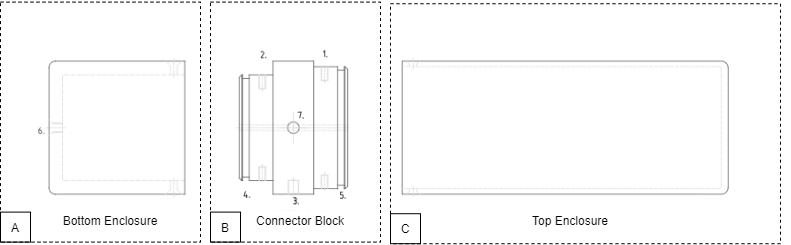
\includegraphics{enclo_schem.PNG}
    \caption{2-D Drawing of the Buoy Enclosure showing the separate components}
    \label{fig:enclo_schem}
\end{figure}

\begin{table}[H]
    \centering
    \caption{Primary Measurements of the buoy enclosure taken from the schematic in appendex \ref{fig:full_schem} \ref{fig:bot_schem} \ref{fig:top_schem} \ref{fig:conblock_schem}}
    \begin{tabular}{||l  l c||}
    \hline
         \textbf{Component} &   \textbf{Dimension} &   \textbf{Value (mm)} \\
         \hline
         \hline
         \multirow{4}{*}{Top Enclosure} & height & 240\\
         &  diameter & 98  \\
         &  wall thickness & 4 \\ 
         & base thickness & 5 \\
         \hline
        \multirow{3}{*}{Bottom Enclosure} & height & 100\\
         &  diameter & 98  \\
         & thickness & 10 \\ 
         \hline
        \multirow{5}{*}{Bottom Enclosure} & height & 80\\
         &  outer diameter & 98  \\
         &  top inner diameter & 89.94  \\ 
         &  bottom inner diameter & 77.85\\
         &  O-ring Thickness & 2.6 \\
         \hline
    \end{tabular}

    \label{tab:enc_meas}
\end{table}

This design allows for easy access to the electronics as well as separation between the various subsystems. The connector block acts as a connection point for the electronics in version 1. This point of contact was a 3d printed connector for a vertically mounted PCB. In version 2, this was replaced by a row of screw holes around the connector block to connect a horizontal Stack of customised PCBs. This was found to greatly improve the robustness of the system and prevented components from breaking. The communication modules, microcontroller and sensors were mounted in the top enclosure while the batteries and power system were placed in the bottom enclosure. The power system was connected to the top enclosure through a drill hole in the connector block. The system was waterproofed by placing 2 o-rings on either side of the connector block. The top and bottom enclosure are fastened to the connector block using a a flat head counter sunk hex screw. Finally a drill hole in the connector block allowed the system to be secured to the buoy stand preventing it from falling out during deployment.

\section{Electronics}

The electronics for the system refer to the Communication subsystems, power electronics, sensors and processors. Due to project time constraints, the approach to developing the platform was to select off the shelf components that satisfied the requirements shown in table \ref{tab:sys_specs}. Further consideration was given to components that were low power (SP011, SP012) and cost effective components (SP013). Additionally, devices with intelligent operations were selected as this would allow us to effectively control the current consumption and operations of the device. These consisted of components with programmable settings such as digital sensors, actuators and modems. The following section gives an overview of the selection consideration for each subsystem

\subsection{GPS}

A Ublox Neo-7m was initially selected as it was easy to procure and has a small form factor. The module comes on a Waveshare breakout board which significantly decreases the development time. The board comes with an active patch antenna which has a gain of about 30dB. In addition, the component is low power with a relatively fast acquisition time and accuracy. The device also can be configured to output diagnostic information and Dilation of procession with the associated measurement which can provide a greater understanding of satelite connectivity in the region. However, by the time we requested more modules, the device was out of stock and had depreciated. To overcome this, we opted for the Neo-M9N module which had significantly improved performance at a higher cost. The table below shows a comparison of the two modules and their key performance parameters.

\begin{table}[H]
    \centering
    \caption{Comparison of key parameters between the initial Ublox Neo-7m gnss module and the updated Ublox Neo-N9M module}
    \begin{tabular}{|l |l |l|}
    \hline
        \textbf{Description} & Neo-7M & Neo-M9N\\
        \hline
         Positional Accuracy: & 2.5m  & 2.0m\\
         Communication Type: & UART, I2C, SPI & UART, I2C, SPI\\
         Cold-Start Time:& 30s & 26s\\
         Supply Voltage & 1.65V - 3.6V & 2.7V -3.6V\\
         Active Current Draw & 32mA &  42mA\\
         Price & R269 \footnotemark & R1,195.45 \footnotemark\\
         \hline
    \end{tabular}
    \label{tab:neo7}
\end{table}
\footnotetext[1]{from Digikey \url{https://www.digikey.co.za/} ordered on 09/2020} 
\footnotetext{from Microrobotics \url{https://www.robotics.org.za/} ordered on 19/12/2018}
The Neo 9-m offers improved performance at a higher cost and higher power consumption. This module comes on a Sparkfun breakout board with an option for an external u.fl antenna or an integrated chip antenna. The chip antenna however has a very small gain making it unsuitable to be used for this application. Therefore, an additional antenna was bought.

\subsection{Iridium}

The Iridium modem is critical for ensuring data can be transmitted from remote locations. When selecting a modem, key considerations were given to the physical size, Bandwidth as well as coverage. In addition, we require a module that is low powered and cost effective. For this reason, we have selected the Rock block 9603 modem which has the following key specifications. This is a module that contains an Iridium 9603 modem on a specially -designed power board. The device communicates via UART with the option for flow control. The module contains a 10-pin picoblade. The module contains 4 communications pins, 1 digital input pin and 2 digital output pins for interfacing with. Power is supplied either through a 5V pin or 3.3V pin in addition to the ground pin. A brief description of the pin out is given in the table below: 

\begin{table}[H]
    \centering
    \caption{Pinout for the Rockblock 9603 Iridium Modem}
    \begin{tabular}{c l l}
        \hline
         Pin Number: & Label & Pin Description\\
          \hline
          \hline
         1 & RXD & UART Output Pin \\
        
         2 & CTS & Flow Control Clear To Send\\
         3 & RTS & Flow Control Request To Send\\
         4 & NetAv & Network Available \\
         5 & RI & Ring Inidcator \\
         6 & TXD & UART Input Pin \\
         7 & OnOff & Sleep Control\\
         8 & 5V & 5V max supply pin \\
         9 & Li-Ion & 3.7V max supply pin \\
         10 & GND & Ground \\
         \hline
         \hline
    \end{tabular}

    \label{tab:ir_pinout}
\end{table}

The device communicates via UART through the RXD and TXD pins. The CTS and RTS pins are optional if flow control is required. The OnOff pin can be used to put the device to sleep which significantly improves power performances. Finally, The NetAv and Ring Indicator are notification pins that can be used to indicate whether there is sufficient signal to transmit as well as to notify when a message is waiting to be downloaded respectively. 

Finally, the key characteristics for the device are shown in the table below:

\begin{table}[H]
    \centering
    \caption{Table showing key parameters and performance characteristics taken from the datasheet}
    \begin{tabular}{|c|c|}
        \multicolumn{2}{l}{Mechanical Features:}\\
        \hline
        \textbf{Antenna: } & Patch or External SMA\\
        \hline
        \textbf{Temperature Rating:} & -40ºC to +85ºC\\
        \hline
       \textbf{Dimensions}  & $45.0 \times 45.0 \times 15.0$ mm  \\
       \hline
        \textbf{Cost: } & R2,850.56\\
               \hline
       \multicolumn{2}{l}{Power Characteristics:}\\
       \hline
       \textbf{Supply Voltage} & 5v or 3.7v Li-Ion \\
       \hline
       \textbf{Start-Up Current} & 450mA \\
       \hline
       \textbf{Active Current} & 100mA \\
       \hline
       \textbf{Sleep Current} & 200uA\\
       \hline
        \multicolumn{2}{l}{Communication:}\\
        \hline
         \textbf{Baudrate} & 19200 b/s \\
        \hline
         \textbf{ Data bits} &  8\\
        \hline
         \textbf{Stop bits} & 1 \\
        \hline
         \textbf{Parity} & none \\
        \hline
        \textbf{Max Upload size} & 340 bytes \\
        \hline
        \textbf{Max Download Size} & 270 bytes \\
        \hline
    \end{tabular}

    \label{tab:ir_specs}
\end{table}

\subsection{Sensors}

2 versions of the buoy were developed from 2019 - 2020 with different sensing capabilities. The first version consisted of a DS18B20 Temperature sensor. This was a low cost, small form factor device that interfaced over One-wire. In version two, this was dropped in favour of the Bosh Sensortech BMP280 sensor. The BMP featured improved sensing capabilities, temperature compensation as well as a programmable interface. In addition, the sensor contains both an ambient temperature sensor as well as a pressure sensor. A comparison of each device is given in the table below

\begin{table}[H]
    \centering
    \caption{Comparison of performance between the BMP280 and DS18B20 environmental sensors.}
    \begin{tabular}{|c|c|c|}
    \hline
         & \textbf{BMP280} & \textbf{DS18B20} \\
         \hline
         Temperature Range & $-40^\circ C \text{ to } 85^\circ C$&$-55^\circ C \text{ to } 125^\circ C$ \\
         \hline
         Accuracy & $1^\circ C \text{ for } T < 0^\circ C$ & $1^\circ C \text{ for } T < 0^\circ C$ \\
         \hline
         Pressure Range  & N/A & 300 to 1100 HPa \\
         \hline
         Pressure Accuracy & N/A & 1.7 HPa $ \text{ for } T < 0^\circ $\\
         \hline
         Price & R87,84 & R85.17 \\
         \hline
    \end{tabular}
    \label{tab:senv_spec}
\end{table}

The BMP 280 is a chip that can be ordered standalone or comes on a I2c/SPI ready breakout board. The device on a breakout board is cheaper than than DS18B20 and can measure both temperature and Pressure whereas the DS18B20 can only measure temperature. The Power characteristics of each device are given in the table below

\begin{table}[H]
    \centering
    \caption{Comparison between supply voltage and current draw of the BMP280 and DS18B20}
    \begin{tabular}{|c|c|c|}
        \hline
         &  \textbf{BMP280} & \textbf{DS18B20}\\
         \hline
         Supply Voltage & 3.0V - 5.5V & 1.71V - 3.6V\\
        Sleep Current & $0.75\mu A$ & $0.3\mu A$\\ 
        Active Current & $1500\mu A $ & $4.2\mu A$\\
        \hline
    \end{tabular}

    \label{tab:env_power}
\end{table}

The BMP280 was chosen for its comparable performance and accuracy. In addition, the BMP280 features more sensing capabilities and is more power efficient and cost effective than the DS18B20 making it suitable for this application.\par 

Finally, a digital sensor for power monitoring was selected to provide constant feedback on the status of the power system. This will be used to monitor the battery voltage as well as the current draw to make sure that the system does not deplete the energy reserves to quickly. To achieve this a INA219A IC was selected and mounted on a custom PCB with a shunt resistor of known resistance. The device has a high reported accuracy of 1\% over a full temperature range and is fully programmable. The device  communicates via I2C with 16-bit registers storing ADC values for  Current (mA),Voltage (V) as well as power (mW). The device is extremely low power with a high voltage measurement range and on-board calibration features. Some key performance parameters are shown in the table below:

\begin{table}[H]
    \centering
    \caption{Performance specifications for the INA219 current monitor chip.}
    \begin{tabular}{|l|l|}
    \hline
         \textbf{Operating Temperature: }& $-40\degree C\text{ to } 125\degree C$ \\
         \hline
         \textbf{$V_{shunt}$ range: }& $40mV \text{ to } 320mV$\\ 
         \hline
         \textbf{$V_{bus}$ rage: } & $0V - 16V \text{ or } 0V-32V$\\
         \hline
         \textbf{ADC Resolution: } & 12-bits\\
         \hline
         \textbf{Measurement Error: } &$\pm 1\%$\\ 
         \hline
         \textbf{Price: } & R17.77\footnotemark\\
         \hline
         \multicolumn{2}{l}{Power Characteristics}\\
         \hline
         \textbf{Supply Voltage: } & $3.3V \text{ to } 5V$\\
         \hline
         \textbf{Quiescent Current: } & $0.7mA \text{ to } 1mA$\\
         \hline
         \textbf{Standby Current: } & $6\mu A \text{ to } 15\mu A$\\
         \hline
    \end{tabular}

    \label{tab:INA_spec}
\end{table}
\footnotetext{source: \url{https://www.digikey.co.za/}}

\subsection{Inertial Measurement Unit}

The MPU6050 is a 6-axis IMU that measures the acceleration and rotational velocity of 3 axes respectively.This component has a small form factor, low power and is fully programmable allowing the device to operate in different modes thereby optimising the data flow to and from the device. While the device does not contain a magnetometer, this is not an issue since the region suffers greatly from magnetic distortion \cite{kohout2015device} thereby rendering all readings to be unreliable. In addition, The acceleration of waves can be defined by the stoke supper limit \cite{kohout2015device} as 0.5g for a non breaking wave. The device has a programmable full scale range for both the accelerometer and gyroscope. IT contains an IIR filter and on-board self testing for added robustness and data integrity thereby making it  the ideal device for this application. The key parameters for the device are shown in the table below:
\begin{table}[H]
    \centering
    \caption{Performance Characteristics of the MPU6050 6-axis IMU }
    \begin{tabular}{|l|l|}
    \multicolumn{2}{l}{Accelerometer:}\\
    \hline
       Full Scale Resolution:  & $ \pm 2g \text{ to } \pm8g$\\
       \hline
        Sensitivity: &  $61.17 \mu g/LSB^{-1} \text{ to } 488.281\mu g/LSB^{-1}$\\
         \hline
        Sample Rate: & 4Hz - 1000Hz\\
         \hline
        Noise Performance: & $400\mu g/\sqrt{Hz}$\\
         \hline
         \multicolumn{2}{l}{Gyroscope:}\\
         \hline
           Full Scale Resolution:  & $\pm 250\degree/s \text{ to } \pm 2000\degree/s $ \\
       \hline
        Sensitivity: &  $7.63(\mu\degree/s)/LSB^{-1} \text{ to } 60.98(\mu\degree/s)/LSB^{-1}$\\
         \hline
        Sample Rate: & 4Hz - 8000Hz\\
         \hline
        Noise Performance: & $0.005(\mu\degree/s)/\sqrt{Hz}$\\
         \hline
         \multicolumn{2}{l}{Device Characteristics:}\\
         \hline
         Temperature Range: & $40\degree C \text{ to } 85 \degree C$\\
         \hline
         Low Pass Filter Range: & 5Hz to 256Hz \\
         \hline
         Supply Voltage: & 2.375V to 3.46V\\
         \hline 
         Active Current: & 3.9mA (Max) \\
         \hline
         Low Power Current: & $< 20 \mu A$ for $ODR < 5Hz$\\
         \hline
         Cost: & R40.00 \footnotemark\\
         \hline
    \end{tabular}
    \label{tab:mpu_specs}
\end{table}
\footnotetext{Source: \url{https://www.communica.co.za/}}

The device has a high range for both gyroscope and imu with ideal low power performances making it the ideal device. In addition, the device comes prototype ready on the GY-521 development board. The device can be interfaced either using SPI or I2C. For this application, the device was interfaced with using I2C.

\subsection{Memory}

Physical memory is an important feature in the device as it allows for permanent storage of data during the life cycle of buoy. Having the device in various sleep modes may result in lost data if the data is stored in RAM.

Flash Chips were selected as a permanent Solution. An array of 4 AT45DB641E SPI Serial Flash Chips were selected and mounted on a PCB directly interfacing with the system. Each chip can hold up to 64Mbit of data. Data can be read/ written at speeds of up to 85MHz of 15MHz in low power mode. The device is low power with high data retention requiring a supply voltage of 1.7V – 3.6V and draws a maximum of 11mA in Active Read mode thereby making it one of the lowest power consumption components in the system. In addition, the device comes with 2 x 256byte buffers that can store data while a read/ write operation is taking place. Memory is Organized into sectors (2 – 256 Kbs long), blocks (2kB long) and pages (256 bytes) with write, read and erase options at each level. The following table shows key performance characteristics

\begin{table}[H]
    \centering
    \caption{Key performance characteristics for the AT45DB641E flash chips.}
    \begin{tabular}{|l|l|}
    \hline
    Operating Temperature:  & $ -40\degree \text{ to }85 \degree$ \\
    \hline
    Storage Capacity: & 64 Mbit \\
    \hline
    Supply Voltage    & 1.7V -3.6V\\
    \hline
     Standby Current: & $45\mu A$ \\
     \hline
     Active Current:  & $22mA$ \\
     \hline
     Unit Cost:       & R 65.307 \footnotemark\\
     \hline
    \end{tabular}
    
    \label{tab:flash_specs}
\end{table}
\footnotetext{Source: \url{https://za.rs-online.com/}}
\subsection{Processor}

For the processor, a single processing unit was selected to reduce complexity of the system. However, in order to satisfy the requirements for the buoy, a processor must be selected with sufficient peripheral ports to handle communication from all sensors, communication modules and memory banks. In addition, there should be sufficient digital input and output pins to control the sensors and provide feedback The communication peripheral requirements are condensed into the following table: 

\begin{table}[H]
    \centering
    \caption{ Type and number of communication ports in order to facilitate communication with  all the external modules.}
    \begin{tabular}{|l|l|}
        \hline \hline
        Peripheral Name: & Qty \\
        \hline \hline
        UART & 2\\
        I2C & 2\\
        SPI & 2\\
        Digital Pins & 11\\
        \hline 
    \end{tabular}
    \label{tab:micro_ports}
\end{table}

Additionally, the processor needs to have a high resolution and large memory bank to handle incoming data. For this reason, a 32-bit micro-controller was identified as the ideal component for the processing system. 3 processors were selected from the STM32 range of microcontrollers and prototyped at various phases during the development cycle. The first version of the buoy contained the STM32F407 which is available on a 100-pin development board thereby decreasing the development time and increasing the technology readyness level of the system. This device was found to have more peripherals than required and had a large power requirement. Therefore the device was replaced by the STM32F446-RE which had significantly reduced peripherals and more optimal performance. The final processor selected was the STM32l476RG. Which matched the STM32F446 in pinout and peripheral however it was significantly more optimised for low power operation. The device had significantly more wake up pins with an extremely low power consumption therefore being the optimal choice. In addition, the development board for the STM32l476 has an on-board debugger which can be removed to reduce the physical size of the device. The STM32L4 can also be configured to passively detect a brownout event as well as a low power event which provides critical feedback regarding the device's performance. Some key performance parameters of the STM32l476 are shown in the table below:
 
 \begin{table}[H]
     \centering
     \caption{Performance parameters for the STM32L4 microcontroller. }
     \begin{tabular}{|l | l|}
     \multicolumn{2}{l}{Electrical Characteristics:}\\
     \hline
      \textbf{Input Voltage: }    & $1.71V \text{ to } 3.6V$ \\
      \hline
      \textbf{Active Current Draw: }    & $100 \mu A/Hz$ \\
      \hline
      \textbf{Shutdown Mode Current Draw: }    &  $30nA$ \\
      \hline
      \textbf{Standby Mode Current Draw: }    &  $420nA$ \\
      \hline
      \textbf{$V_{brownout}$ Threshold:} &  $1.66V \text{ to } 2.90V$\\
      \hline
       \multicolumn{2}{l}{Computational Characteristics:}\\
     \hline
     \textbf{Processor: }    &  ARM Cortex-M4 \\
     \hline
     \textbf{MCU Size: }     & 32-bit\\
     \hline
     \textbf{Float representation: } & Hardware FPU \\
     \hline
     \textbf{Flash size: } & 1MB\\
     \hline
     \textbf{RAM Size:} & 128 KB\\
     \hline
     \textbf{Clock Source: } & LSE, HSE, LSI, MSI, HSI \\
     \hline
     \textbf{System Clock Frequency: } & 4MHz to 80MHz \\
     \hline
     \textbf{Dhrystone Benchmark: } & 1.25 DMIPS/Hz \\
     \hline
     \multicolumn{2}{l}{Communication Ports:} \\
     \hline
     \textbf{Total  Communication ports: } & 20 \\
     \hline
     \textbf{UART Ports} & 5 \\
     \hline
     \textbf{I2C Ports} & 3 \\
     \hline
     \textbf{SPI Ports} & 3 \\
     \hline
     \end{tabular}

     \label{tab:stm_spec}
 \end{table}
 
 The STM32l4 also features seven general purpose timers as well as two advanced timers and two low power timers. In addition, the device has five wake up pins which allow the device to be woken up from deep sleep (shutdown) via an external source. The device is capable of DSP processing using external libraries provided by the manufacturer and a real-time clock thereby making it the ideal component to be a processor for the buoy.
 
 \subsection{Power Electronics}
 
 Based on the aforementioned Hardware selection, the following power requirements are outlined in the table below:
 
 \begin{table}[H]
     \centering
      \caption{Current consumption of various components as well as the estimated maximum possible current draw}
     \begin{tabular}{|c|c |c|c|}
         \hline
         Device Name & QTY &  Supply Voltage & Maximum current Draw\\
         \hline
         Ublox NEO-M9N & 1 & 3.3V & 42mA \\
         \hline
         Rockblock 9603 & 1 & 5V &  450mA\\
         \hline
         BMP280 & 1 & 3.3V & 0.0042mA\\
         \hline
         INA219A & 1 & $V_{Bat}$ & 1mA\\
         MPU6050 & 1 & 3.3V & 3.9mA\\
         \hline 
         AT45DB641E & 4 & 3.3V & 88mA\\
         \hline
         STM32L476RG & 1 & 5V & 2.6mA\\
         \hline
         \cline{4-4}
         \multicolumn{2}{c}{} &\multicolumn{1}{c}{\textbf{total:}} & \multicolumn{1}{c}{587.50mA} \\
         \cline{4-4}
         \cline{4-4}
     \end{tabular}

     \label{tab:pow_budget}
 \end{table}
 
 From table \ref{tab:pow_budget} we can expect a maximum current draw of 587.50. The largest consumer of power is the Rock-block 9603 which can draw up to 450mA when charging. Therefore, the power supply needs to be able to supply at-least 500mA during start up. Current can be conserved by placing the devices into sleep mode which further reduces the current consumption from the batteries. Finally, By only turning the components on when required, even less power can be conserved. \par 
 
 Therefore, a regulator is required that is capable of supplying the required current  while being able to stand the drastic changes in current consumption. A decision was made to use a 5V low Dropout regulator to supply the 5V components directly i.e. the iridium modem and the micro-controller. The 3.3V components are powered through the on-board 3.3V regulator for the STM32L4 nucleo development board. The Low Dropout regulator is a LP3876 7V LDO capable of supplying up to 3A. The device has a quick response to step changes and an adjustable output voltage thereby making it the ideal device to supply power. The output voltage level can be controlled by selecting capacitors. For this application a $10 \mu C$ tantalum capacitor was used as tantalum capacitors have  excellent robustness and transient responses especially at low temperatures.  Some key characteristics for the device are given in the table below
 
 \begin{table}[H]
     \centering
      \caption{Key Performance Characteristics for the LP3876 Low Dropout Regulator}
     \begin{tabular}{|l|c|}
     \hline
          Input Voltage & $2.5V \text{ to } 7.0V$  \\
          \hline
          Voltage Regulation (over current)& 0.14\%\\
          \hline
          Dropout Voltage at 3A & 0.8V to 1.2V  \\
          \hline
          Quiescent Current at 3A &  14mA\\
          \hline
          Temperature Range & $-40 \degree C \text{ to }125 \degree C$\\
          \hline
          Unit Cost & R95.19 \footnotemark\\
          \hline
     \end{tabular}    
     \label{tab:lp_spec}
 \end{table}
 
 \footnotetext{source: \url{https://www.digikey.co.za/}}
 
The LDO was placed on a customised PCB  with the INA 219 Current sensor as well as an indicator LED to show that the batteries have sufficient charge. The power board was supplied by 3.6V C-cell LiSOCl2 batteries. These batteries have ideal low temperature characteristics as well as a high capacity. 2 cells were placed in series to create a 7.2V power source which was placed in parallel with another 7.2V array to increase the capacity. The batteries, battery holders and power board are connected to form a single subsystem which was placed in the bottom enclosure and connected to the micro-controller via a 7-pin cable.

\section{Final Assembly}
\label{sec:ch3_final_assembly}
The final electronics choice and configurations are shown in the figure below:

\begin{landscape}\centering
\vspace*{\fill}
\begin{figure}[htpb]
  \centering
  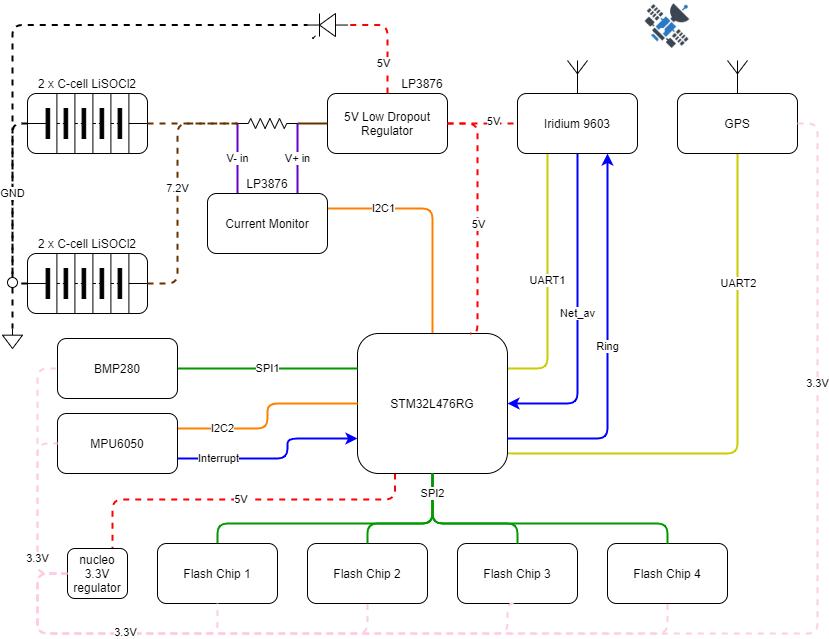
\includegraphics[height=0.6\textheight, width=1.2\textwidth]{figs/SHARC_Final.png}
  \caption{Simplified schematic of the final version of SHARC buoy showing power supply (dash), communication (solid) and digital connections (arrows) and configurations}
    \label{fig:sharc_final}
\end{figure}
\vfill
\end{landscape}


A final costing of the system is provided in the table below:
\begin{table}[H]
    \centering
    \caption{Approximate procurement cost for a single SHARC buoy node.}
    \begin{tabular}{l c r r}
    \hline \hline
        \textbf{Component Name:} & \textbf{QTY:} & \textbf{Unit Cost} & \textbf{Total:}  \\
        \hline \hline
        Buoy Enclosure and Stand  & 1 & R1,206.84 & R1,206.84 \\
        Ublox Neo-M9N & 1 &  R1,195.45 &R1,195.45\\
        Rockblock 9603 & 1 & R3,278.144 & R3,278.144 \\
        M1621HCT Helical Antenna & 1 & R1,411.15 & R1,411.15 \\
        BMP280 & 1 & R46.00 & R46.00 \\
        INA219A & 1 & R17.77 & R17.77 \\
        MPU6050 & 1 & R40.00 & R40.00 \\
        AT45DB641E & 4 & R65.307 & R261.229 \\
        Nucleo-l476RG & 1 & R215.98 & R215.98 \\
        Fanso C-cell 9000mAh Battery & 4 & R101.81 & R407.24 \\
        BHC-2ND Battery Holder & 4 & R61.87 & R247,48 \\
        LP3876 5V regulator & 1 & R95.19 & R95.19 \\
        Wiring and Connectors & - & R136.46 & R136.46 \\
        \hline 
        \hline
        & & \textbf{ Grand Total: } & R8,421.13\\ 
        \hline \hline
    \end{tabular}
    \label{tab:total_cost}
\end{table}

Customised PCBs were designed to connect the various subsystems together. The device was kept modular by separating PCBs and grouping devices by functionality. A circuit board was created for the Dropout regulator and INA219 current sensor which was affixed to 4 x C-cell battery holders.The battery holders have leads which were were arranged in a 2-series, 2- parallel configuration.

\begin{figure}[H]
    \centering
    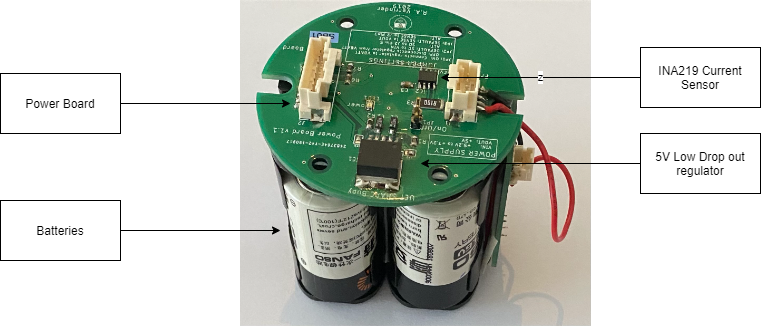
\includegraphics[scale = 0.5]{bot_encl.png}
    \caption{Power Module for the SHARC BUOY. A custom PCB with Dropout Regulator and current sensor connected to a battery pack}
    \label{fig:bot_elec}
\end{figure}

This module was placed in the bottom enclosure and fastened to the connector block using a hex screw. A customised 7-pin duraclick cable connects the module to the modules in the top enclosure. A main connector board was developed with duraclick connections for each of the aforementioned devices. The board contains 2  2x16 female header rows to fit the morpho connectors of the nucleo-l4 development board. 2 more disc-shaped PCBs were developed. First a communication boards which contains a 4-pin female header to connect the ublox GPS module and 2 brackets to mount the iridium module vertically. A helical antenna connects to an SMA antenna on the Iridium module. Then a sensor board for the IMU and environmental sensor. The boards were connected in a stack configuration and fastened to the connector block using M6 metal Hex Spaces with the communication board being placed at the top for direct line of sight with satellites. The environmental board was secured to the base of the connector block with the BMP280 placed face-down over a hole drilled through the connector block allowing it to interface with the environment.
 \begin{figure}[H]
     \centering
     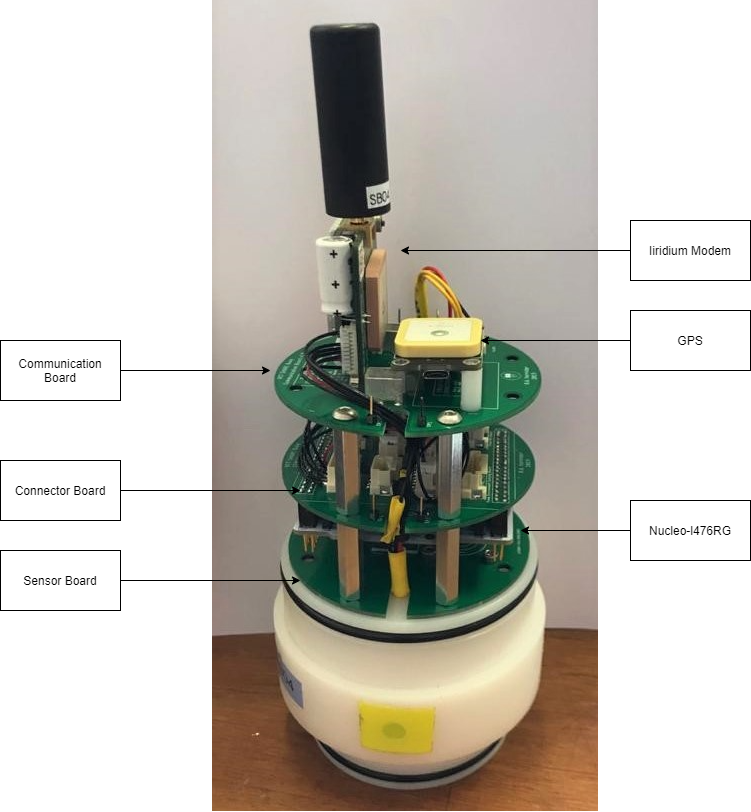
\includegraphics[scale =0.5]{Top_encl.png}
     \caption{Electronic Stack for the top module consisting of connector board, micro-controller board and sensor board attached to the connector block }
     \label{fig:top_elec}
 \end{figure}

This configuration greatly increases the robustness of the electronics and can overcome breaking caused by poor handling or improper deployment.  The top enclosure is placed over the electronics and fastened to the connector block using Hex screws. Finally, the system is placed in the stand housing and secured using another hex screw.

\begin{figure}[H]
    \centering
    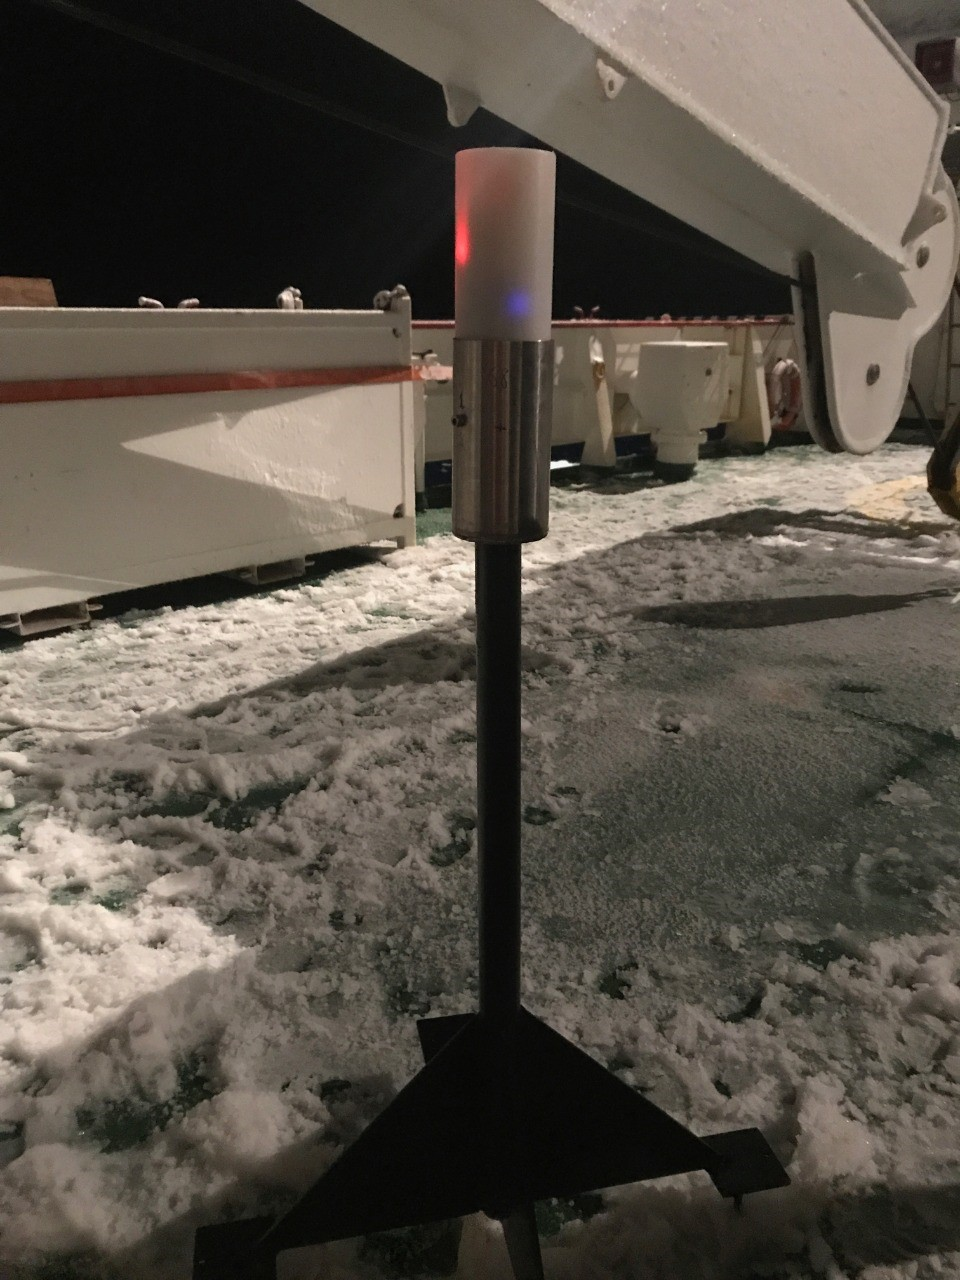
\includegraphics[scale = 0.5]{full buoy.jpg}
    \caption{SHARC BUOY fully assembled and in deployment state. Electronics placed in enclosure and fastened to the buoy stand. LEDs on the various components indicate that the device is in working order}
    \label{fig:my_label}
\end{figure}

\chapter{Software Design}
\label{sec:ch3_soft}
This section outlines the design methodology for the SHARC Buoy Software. The software cycle was designed with consideration towards the IEEE software standard 12207.1\footnotetext{Software life cycle processes—Life cycle data\cite{IEE_STD_SOFTCYCLE}}.


The software structure was kept as compartmentalised as possible to improve the modulator of the firmware. This would allow for fewer changes to be made during the design process allowing for a quick response to hardware changes. The design process was iterative as changes were made over the design cycle to the micro-controller platform as well as the sensors. In addition, some of the required libraries had depreciated and needed to be replaced.  This section will focus solely on the firmware design for the overall system as well as the subsystem. 

This section begins with an overview of the development environment which discusses the tools, platform and any libraries that were used. Then an overview of the main firmware is given. Each aspect of the system is described in terms of function, configuration parameters as well as location in the overall scope.

\section{Software Architecture}

The STM32 series does not come loaded with any Operating System. Therefore, firmware development had to occur on bare metal. In addition, the firmware had to be tailored to the specific micro-controllers architecture. The Atollic Truestudio IDE allowed for development to take place in C. The program comes packaged with an ARM development tool chain and a C compiler allowing for code to be compiled and flashed onto the board via a USB cable. The manufacturer also provides a set of driver files and  initialisation tools. The project was written in C which allowed for higher-level code to implemented while still optimising for size and speed on the device. In addition, C allows for the program to include drivers and resources from the manufacturer. \par 

The Firmware was designed using a top down approach. The overall system was decomposed into 3 distinct layers as shown in the figure below

\begin{figure}[H]
    \centering
    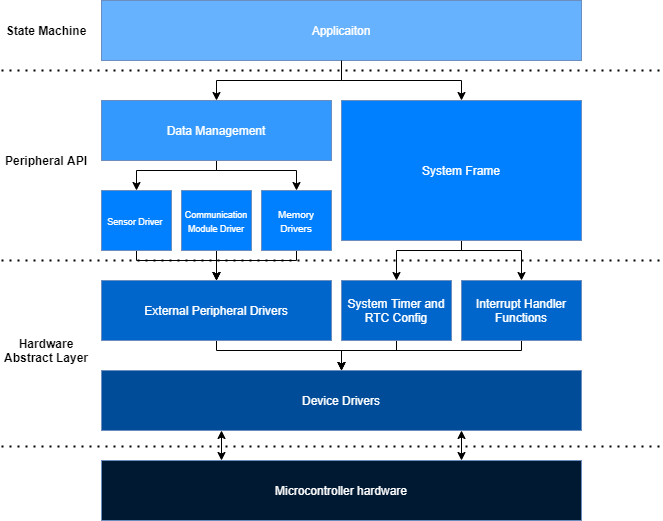
\includegraphics[width= 0.7\linewidth]{soft_arch.png}
    \caption{Diagram showing the decomposition of the overall firmware into distinct layers and the relationship between each part.}
    \label{fig:soft_arch}
\end{figure}

The Hardware Abstract layer consists of the driver files used to initialise and control the hardware of the micro-controller.This layer is platform specific therefore needs to be tailored to the architecture of the micro-controller. The manufacturer provides hardware driver files which were used to form the Hardware abstract Layer.The Standard Peripheral Library (SPL) was used in the first version of the firmware however, the library had depreciated and was replaced with the Hardware Abstract Layer (HAL) libraries. HAL libraries were used to form the foundation of the code as it allows for the code functionality to run independently from the hardware architecture. Should a new micro-controller be required, the HAL library simply needs to replaced. Therefore allowing the firmware to maintain modularity and increase portability. In addition, the HAL Library offers robust error checking and flagging. If a peripheral fails at any point during run time, the libraries provide handlers and flag signalling to handler the error. \par 
Once The HAL Layer was finished, customised driver files were written for each module. These files were written to interface with the sensor through the HAL layer thereby reducing dependencies on the hardware, in addition, these driver files were created to abstract the initialisation and configuration process of each peripheral as well as the hardware routines that occur. In addition, some external modules required the use of more than one peripheral such as timer channels for input capture or GPIO pins for External interrupt detection. Finally, these drivers are critical for managing the flow of data too and from the module. The files contain functions that interpret incoming data bytes and convert them to the relevant data type.

\par 

Finally, driver files, configuration files and other libraries are synthesised and sequenced into one main program. This program calls the functions defined in the Driver files. This program provides a frame for the various modules to interact with system. This will be discussed in greater detail in the section below

\section{Project Structure}

The project was set up using CUBEMX for creating peripheral initialization and handling functions. Final code for the project can be found in the folder BUOY\_Frame\_L4. All the tools, definitions and functions developed for the Buoy frame have been organised into the library files Sharc\_Frame.h and Sharc\_Frame.c. This allows for the frame to ported over multiple projects allowing for a new firmware version to be developed from scratch instantly.
The project code files are organised into the following folders:

\begin{enumerate}
    \item Drivers
    \item src
    \item Start Up
\end{enumerate}
The project code files are organised into the following folders:
1.	Drivers 
2.	SRC
3.	Start Up
The Drivers folder contains the HAL and CMSIS libraries for the device.  The SRC Folder contains the main.c file which acts as the entry point for the program to run. The start up file contains assembly code that specifies the vector table, Hard fault/ Reset Handler Entry Points as well as the entry point for the main code. When the file startup\_stm32l476xx.s is run, the program enters into the main() function and begins running from there. The SRC folder contains the .h/.c pair Sharc\_Frame files which are implemented in the main.c 
The main() code consists of a set up phase and a loop phase. During the set-up, the functions HAL\_Init(); and SystemClock\_Config(); are used to reset the peripherals and the systick timer and set the System clock to the correct source and speed. These two functions run in the set-up phase of the code and are called whenever the program re-enters the main function. The next step in the set up phase is to configure the unused GPIO pins to analog floating mode. This greatly reduces the current consumption by the micro controller. The peripherals required for debugging the code are placed here. Before deployment, the code will be removed. This phase is referred to in the program as the System Init and Clock Configuration. It is the first phase to be run.
The next phase in the Set-up is the Power and Reset State Check. If any power event occurs, a software reset is generated, and the program will restart from the main() function. When this happens, a flag is set in the RCC\_CSR. This can occur in the form of a brown out, Pin reset or Low Power event. This phase will check for the occurrence of any event and handle them before the program enters the main loop. Finally, if successful the program will enter the main loop and the firmware will begin.  

\subsection{Power Mode Selection}

 The focus on development optimizing for power consumption as well as accuracy. The system requirements are extremely flexible since the required sampling rate is very slow for example, the largest consideration of the system is Accelerometer sensing which has a maximum expected sample rate of 100Hz. For this reason, high speed computing techniques are not required and do not require much optimization. Since the system will most likely be in a wait state for the majority of its operation, It is important to place the device in as low power mode as possible to minimize consumption. This will be elaborated on in the following sections
The biggest Consideration with system operation is clock speed and source. The STM32l4 has 5 possible options: 3 internal oscillators (MSI,LSI,HSI) and 2 external crystal oscillators (HSE and LSE) these clock sources will provide power to the peripherals as well as the RTC. According the reference manual, the real time clock must be clocked from the LSE 32.768KHz crystal in order to provide an accurate calendar function therefore, the RTC must be clocked from the LSE no exceptions. The external crystal oscillators provide high precision clock speed with extremely low drift however, the power consumption of these oscillators are much higher than the internal RC. The clock configuration of the STM32L4 allows for a combination of these oscillators in a Phase Locked Loop (PLL) which allows for a greater degree of accuracy at desired speeds. 

\begin{figure}[H]
    \centering
    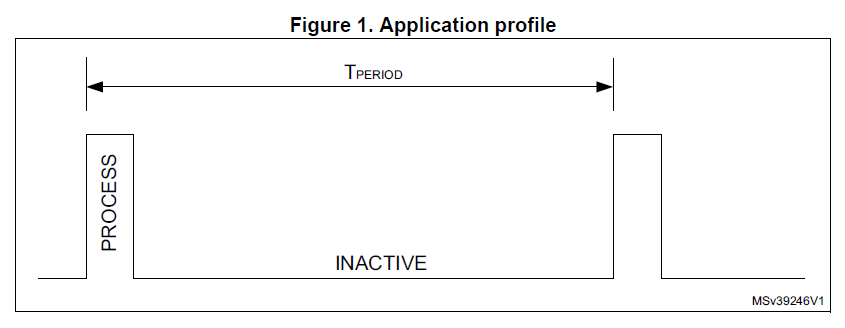
\includegraphics[scale= 0.6]{Application profile.png}
    \caption{Diagram showing a general low power operation profile  for the micro controller with two distinct phases: Process and Inactive occuring over a period T}
    \label{fig:appr}
\end{figure}

Figure \ref{fig:appr}

above details a typical low power operation Which can be expected from the buoy For a typical application, we consider two main phase:
\begin{enumerate}
    \item Process phase: System is in run mode with peripherals are active at regular intervals.
    \item Inactive phase: System is asleep until RTC/GPIO event.
\end{enumerate}

Once the buoy has finished an active routine, the system becomes inactive between samples. The buoy is designed to operate in routines occurring once every half an hour. Once the routine is complete, it still has to wait an extremely long time before it is required again. This is the inactive between sample mode and consider this our period of inactivity where we can place the device in the lowest possible state with very little concern for wake-up time or peripheral settings. \par 
Therefore, the following power modes were selected for each phase of the system's operation

\begin{table}[H]
    \centering
    \caption{Table showing the power mode selection for each phase of the Buoy's operational cycle}
    \begin{tabular}{|c|c|c|}
    \hline 
        Phase &  Power Mode & Current Draw \\
        \hline
        Process & Run Mode & 1.16mA\\
        Inactive & Standby Mode & 710nA\\
        \hline
    \end{tabular}

    \label{tab:powmode_cycle}
\end{table}

Table \ref{tab:powmode_cycle} above shows the estimated current consumption taken from the STM32L4 datasheet. The Current Value for Run Mode was bench-marked using a Dhrystone Test with an system clock of 24MHz and code loaded from Flash. The Inactive current draw was estimated with a Low Speed External Oscillator supplying the Real Time Clock. 

\subsection{Clock Selection}

The biggest Consideration with system operation is clock speed and source. The STM32l4 has 5 possible options: 3 internal oscillators (MSI,LSI,HSI) and 2 external crystal oscillators (HSE and LSE). Since the buoy will be inactive for long periods of time, an accurate 1Hz reference signal is required to keep calendar date and time. In addition, The STM32 microcontroller features a variety of wake up options to transition from low power mode to run mode
\begin{enumerate}
    \item Internal  configurable Alarm
    \item Periodic Wake Up Alarm
    \item External Wake Up Pin
\end{enumerate}

These options are made available through an internal Real Time Clock on the STM32L4 microcontroller. The peripheral can receive input from multiple clock sources such as an external Low Speed Oscillator (LSE), an internal Low Speed Oscillator (LSI) or an internal High-speed Oscillator (HSI). The peripheral also allows for fast and simple data storage during extreme power down modes. When the device enters shutdown mode, RAM is turned off, therefore all data will be lost. The RTC has 32 back up registers capable of retaining 1Kb of data when the device is powered down. \par 

these clock sources will provide power to the peripherals as well as  According the reference manual, the real time clock must be clocked from the LSE 32.768KHz crystal in order to provide an accurate calendar function therefore, the RTC must be clocked from the LSE no exceptions. The external crystal oscillators provide high precision clock speed with extremely low drift however, the power consumption of these oscillators are much higher than the internal RC. The clock configuration of the STM32L4 allows for a combination of these oscillators in a phase locked loop (PLL) which allows for a greater degree of accuracy at desired speeds. The final clock configuration parameters are shown in the table below:

\begin{table}[H]
    \centering
    \caption{configuration parameters for the system clock and Real Time Clock including sources and frequencies}
    \begin{tabular}{|l|l|}
    \hline
    Run Mode System Clock Source: & MSI and LSE in a PLL Configuration \\
    \hline
     Clock Frequency: & 24 MHz \\
     \hline
     Shut Down Mode Clock Source: & LSE \\
     \hline 
     RTC Clock Frequency & 1 Hz \\
     \hline 
     LSE Clock Frequency  & 32.768 KHz \\
     \hline 
    \end{tabular}
    \label{tab:clock_conf}
\end{table}

\section{Firmware Overview}

In a multi-sensing system, it is important to manage the interactions and data flow between the various aspects of the system to ensure the device operates in a predictable, manage manor. To achieve this, a state machine can be implemented to provide a high-level form of control over the system. This can be achieved by decomposing the overall function of the buoy into a series of finite states. These states are connected through a series of transitions which can be described using Boolean techniques. Through this, the buoy retains a modular structure both in firmware and in hardware which can allow for additionally sensors and functions to be implemented seamlessly.\par 


\subsection{Execution}

The goal of the buoy is to sample environmental, GPS and power data at a fixed rate. This rate $T_{sample}$ will be used to describe the period between sampling the devices. Each Sample will be condensed into a byte packet and stored in flash memory at a sector. After every 4 samples, the device will load the packets from memory into a buffer and transmit the data. When the device exits this state, it will reset the sample count and repeat until the buoy is turned off or loses power. The buoy can therefore be broken down into a set of finite states which are shown below:

\begin{enumerate}
    \item \textbf{Initialisation State:} The device initializes the counter and verifies the sensors.
    \item \textbf{Reset State:} Counter and memory Variables are Reset
    \item \textbf{Sample State:} During this state, the device actively receives data from the sensors and stores them into a packet which is then saved to Memory
    \item \textbf{Sleep State:} The device enters this state between samples and active states. Here, the device will remain in this state for a time $T_{sample}$. After which, the buoy will wake up 
    \item \textbf{Transmit State:} The device will load the data from memory and transfer to the Iridium Modem Buffer. Upon successful transmission, it will enter the Reset state
\end{enumerate}

Each state will control which routines are performed during the function and provide the system with information on the current status of the device. Should the device encounter a hardware reset, the system can recover and predict the action it needs to take based on the last state the system was in. A typical system run is shown in the figure below:

\begin{figure}[H]
    \centering
    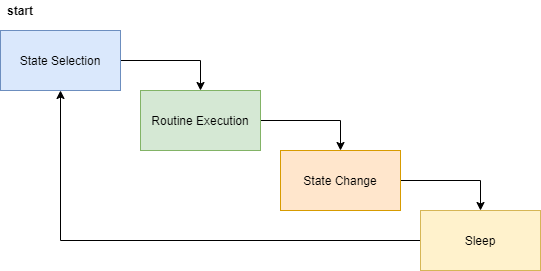
\includegraphics[scale = 0.5]{state Run.png}
    \caption{Diagram showing the steps executed from wake up when }
    \label{fig:state_run}
\end{figure}

The inputs to the state machine are:
\begin{enumerate}
    \item C: a 2-bit integer signifying the number of samples performed $(0 \leq N <4)$
    \item T: Variable that matters when the system is asleep. Signifies whether the system has been in sleep mode for a time defined by the constant value $T_{wake}$
\end{enumerate}

The system has no explicit outputs however, the state machine is used to control which routines will be executed during the execution phase of the program. Therefore, the outputs can be considered as the Routine Rx as shown below:
\begin{enumerate}
    \item $R_{sample}$: Sensor sample routine, this can involve all the sensors or just a select number. For simplicity's sake, this period implies all sensors will be sampled from
    \item $R_{sleep}$ : Device is in a sleep state and will wake up when the periodic wake up unit counts to a time $T_{wake}$
    \item $R_{Transmit}$ : Satellite Transmission Routine
\end{enumerate}

Given the following information, the Algorythmic State Machine (ASM) chart is derived and shown in the figure below

\begin{figure}[H]
    \centering
    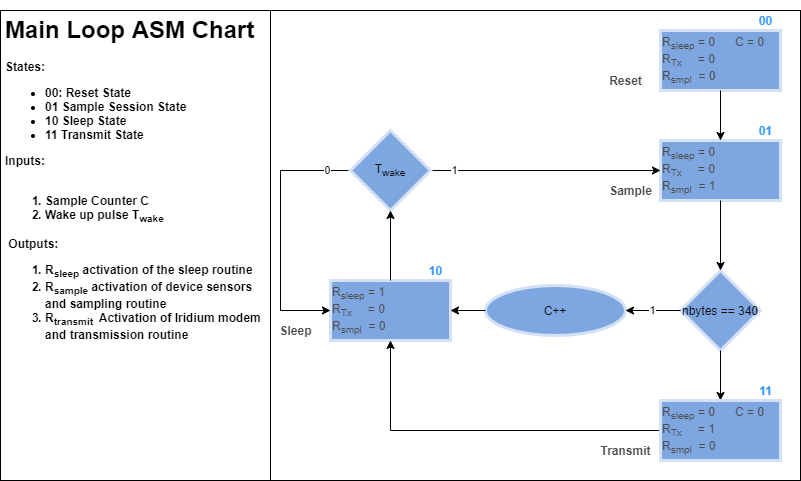
\includegraphics[scale=0.6]{Main Loop ASM Chart.png}
    \caption{ASM chart for the proposed program to run on the processor showing entry/exit conditions and functions to be run during states.}
    \label{fig:ASM_chart}
\end{figure}

Figure \ref{fig:ASM_chart} above shows an abstract representation of the logical flow of the program. A typical run from the system will have the buoy initialised and calibrated before entering the main loop where it will alternate between active sampling and inactive sleep mode until enough data has been collected to transmit. This allows the Iridium modem to only be turned on when needed thereby significantly conserving energy while allowing for the system to sample as much as possible. The variable $T_{wake}$ is user defined and sets the sample rate of the system For this application it has been set to 30 minutes. The device will sample 4 times with 30 minute intervals in-between and transmit the data on the 4th cycle i.e. every 2 hours.

The RTC periodic wake up unit is used as a counter in deep sleep mode. This is a 16-bit down-counting Auto Reload Register that generates an interrupt on an internal wake up line when the system has Slept for a length of time T as defined by the user. In addition, the sample counter gets reset after every transmission state and when the buoy enters a reset state. The number of samples before transmission is chosen to be 4 to optimize packet size for the transmission buffer. Since the Iridium Buffer is 340 Bytes long and the Transmission rate is per 50 bytes, the goal is to transmit as much data that would fit into the buffer as possible. Too frequent transmissions incur a high data cost but result in data integrity. Too few transmissions can result in lost sample points if a transmission is not received.

\subsection{Asynchronous Behaviours}
Asynchronous behavior describes all functionality that occurs outside of the main loop. This can come from Interrupts/ External events which causes the system to exit the main loop regardless of state and execute the code. This can occur from the following sources:

\begin{enumerate}
    \item Interrupts
    \begin{enumerate}
        \item Iridium Message Received (Ring Alert)
        \item IMU Event Detection (Collision / Free-fall detection)
    \end{enumerate}
    \item Events
    \begin{enumerate}
        \item Low power detection.
        \item Brown out detection.
        \item Software resets.
        \item Watch Dog resets.
    \end{enumerate}
\end{enumerate}

These events take precedence over the main loop function. The table below shows the entry/exit conditions. Functionality as well as return state after exit. A full description of events, interrupts, and the protocols for handling them are shown in tables \ref{tab:Int_desc_RI} to \ref{tab:Ev_desc_SWR} in Appendix \ref{sec:evt}. The figure below shows how the event handling procedure is sequenced in the main program:

\begin{figure}[H]
    \centering
    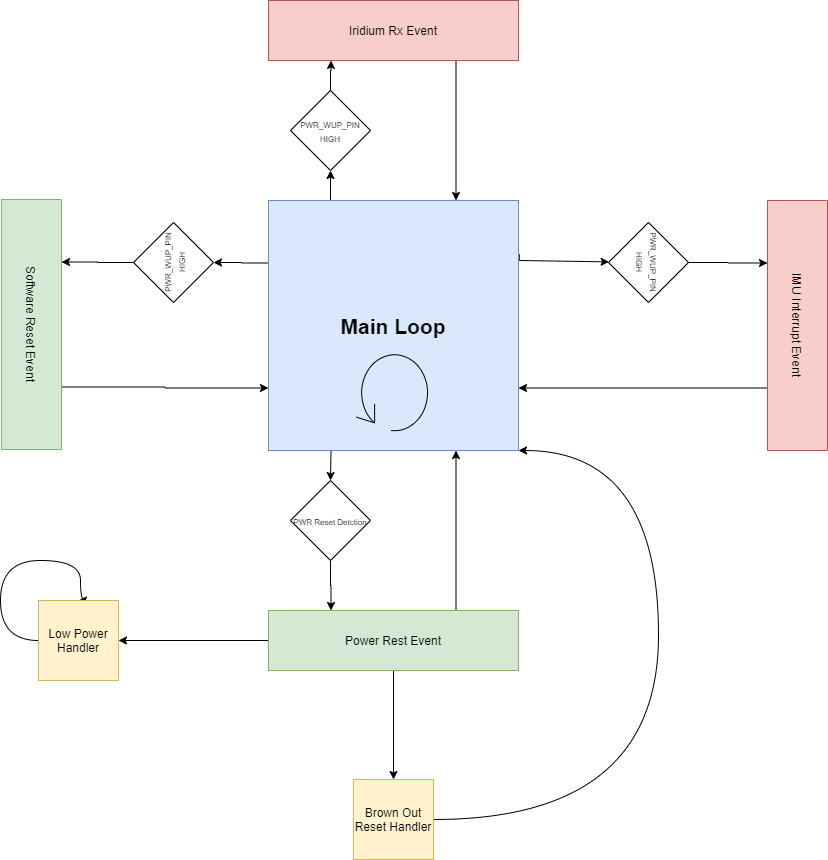
\includegraphics[scale=0.4]{Asynchronous State diagram.png}
    \caption{Application Diagram with Event and Interrupt sequencing}
    \label{fig:main software}
\end{figure}

States are represented by integers on the system and are stored in the back up registers of the RTC. These registers keep data even when the device is in low power mode or a software reset has occurred therefore making them the perfect storage location. The State Variable holds the value of the current state of the buoy. This variable is stored in two locations: When the system is in run mode, the value is stored in the global variable \textit{Current\_State}. When the device is in a deep sleep state, The variable is stored in the RTC Back up registers at byte 0 of Back-Up Register 0. Upon wake up, the value is loaded from the register and placed in the global variable.

The main loop follows a sequential state transition as described in Figure \ref{fig:main software}. To achieve this, at the start of each loop, the program reads the value stored in the state variable. This determines what the previous state was. Based on this value, the new state is determined and stored in the state variable. This process is shown in the figure below.

\begin{figure}[H]
    \centering
    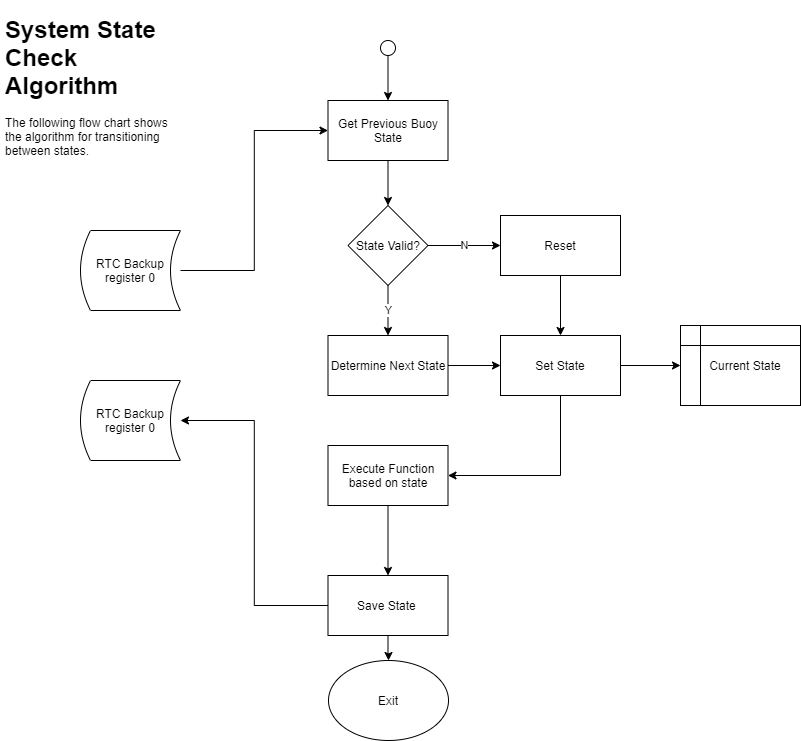
\includegraphics[scale=0.5]{State Check Algorithm.png}
    \caption{Flow chart for the state-check algorithm}
    \label{fig:state_check}
\end{figure}

Figure \ref{fig:state_check} above shows the algorithm for selecting and transitioning between states. This algorithm allows for states to be linked in any order and, most importantly, Separates the state selection from the state function. By separating these two concepts, a more modular framework is created. This allows for the addition of more states and transitions without modifying the routines that are currently in place. This allows for device functions to be turned on and off as desired without drastic changes to the firmware.

Finally, Asynchronous States take a higher precedence over the main loop states and therefore are checked before the state check shown above. The order of precedence is shown in the table below:
\begin{table}[H]
    \centering
    \caption{Table showing the types of states that the system checks for ordered by priority with 1 being the highest priority and 3 being the lowest}
    \begin{tabular}{|l|c|}
         \hline
         Name & Priority \\
          \hline
         Power Event & 1 \\
         \hline
         Asynchronous Interrupt & 2 \\
             \hline
         Sequential State & 3 \\
             \hline
    \end{tabular}

    \label{tab:state_prio}
\end{table}

Power Events generate a system reset and raise a flag in the PWR Status Register. When the flag is set, the program enters the handler and, if the event is non-fatal, returns to the main loop. The following flow chart shows an example of such a case for a Brown Out Event

\begin{figure}[H]
    \centering
    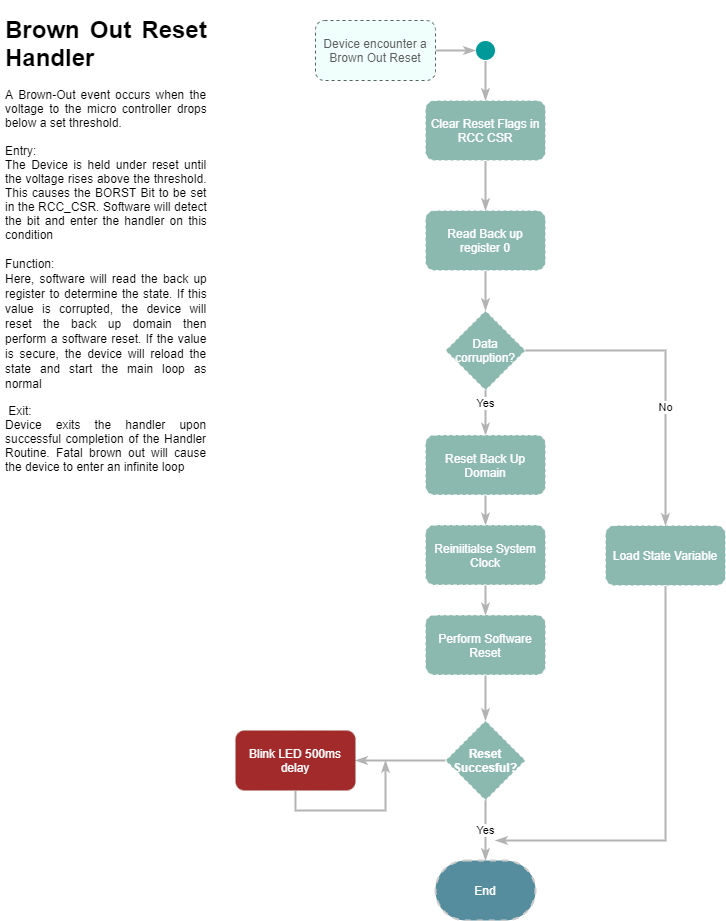
\includegraphics[scale = 0.4]{Brown Out Reset Handler Flow Chart.png}
    \caption{Diagram showing the algorithm for Brown Out Event Recovery and Handling}
    \label{fig:evt_handle}
\end{figure}

Some sensors have interrupt pins and can be configured to trigger upon detection of a specific event. When this happens, the sensor will send a digital high on the interrupt pin. On the processor side, a hardware interrupt is generated and the software handles the interrupt. An example of such a prceedure is shown in the figure below

\begin{figure}[H]
    \centering
    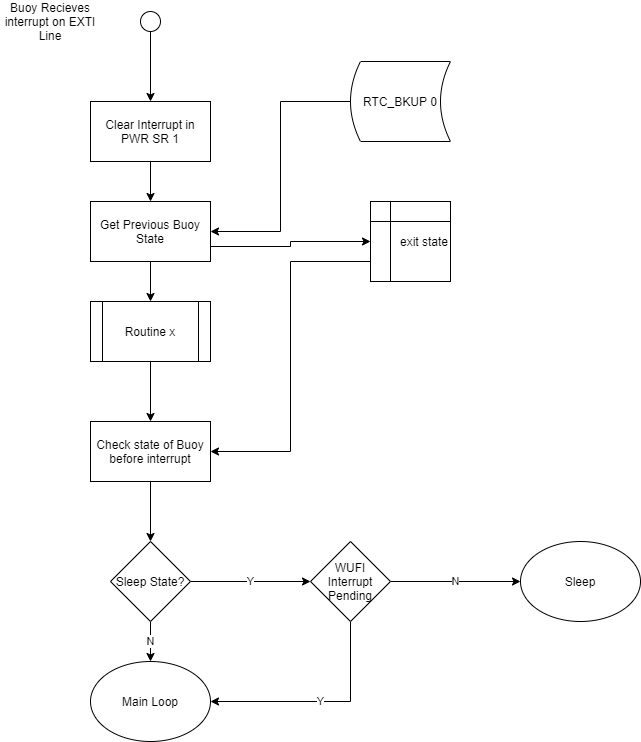
\includegraphics[scale = 0.5]{Asynchronous State flow chart.png}
    \caption{Diagram showing the algorithm for handling an external interrupt from a Wake Up pin connected to one of the modules}
    \label{fig:int_handle}
\end{figure}

By connecting these pins to external wake up pins, the buoy is capable of event detection in deep sleep mode. If an event is detected while in deep sleep, the interrupt causes the buoy to wake up and resume from the beginning. No interrupt handler is entered at this point. A flag is set the PWR\_SR at the position of the wake-up pin it detected. The buoy will enter the asynchronous state depending on which flag is set and will execute the routine associated with it.  When the buoy wakes up from an internal wake up timer, the pins are reconfigured into GPIO EXTI mode which allows the buoy to receive interrupts when active. Note: by keeping the buoys configured as wake up pins, the system will reset when an interrupt is detected.

\subsection{Subsystem Execution}

When a module is is being used at any point in the program. The micro-controller will execute an initialise routine. This will enable any required peripherals for communication with the subsystem. This function will be called before every sample period in case the system encounters a power surge or an unexpected reset. Additionally, placing the micro controller in deep sleep mode results in the registers being reset upon wake up. The initialisation routine is specific to each micro-controller and includes the following:

\begin{enumerate}
    \item High Level Communication Peripheral Configuration
    \item Low Level Pin configuration
    \item Sensor Verification function
    \item Sensor Configuration function
    \item Return Status
\end{enumerate}

The outcome of the initialisation routine is evaluated based on a return status from the function. Items 1 - 3 are included to configure the subsystem to adhere to the functional requirements in table \ref{tab:sys_specs}. Sensor Verification functions are included to satisfy acceptance Tests AT001 and provide evaluations for acceptance tests AT002 and AT004. The initialisation function is designed handle fail modes by evaluating the system's failure return type and responding in accordance with the protocols outlines in acceptance Test 2. Initialisation routines for each subsystem is provided in Appendix \ref{fig:Init_diagram_gps} to \ref{fig:Init_diagram_mpu}

If the initialisation was successful, the program will continue using the module in the firmware. Should a failure occur, the system will attempt to reconnect with the device a predefined number of times. In case of a critical failure, the system will acknowledge that it can no longer use the device and will continue the main firmware without it. The resulting behaviour is shown in the table below:

\begin{table}[H]
    \centering
     \caption{Table Showing the device behaviour in case of a critical failure in one or more of the subsystems. Critical failures are defined in AT006 (table \ref{tab:AT006}) testing protocol.}
    \begin{tabular}{|l|l|l|}
    \hline
       \textbf{Device Failure Case:}  & \textbf{Impact:} & \textbf{Result:}\\
       \hline
       Iridium & Critical & No data will be transmitted from the buoy \\
       \hline
       Flash Chips & Critical & Data will be lost when power is reset \\
       \hline
       GPS & High & GPS data will not be captured \\
       \hline
       MPU6050 & High & Unable to measure Waves in Ice  \\
       \hline
       Environment Sensor & Medium & Environmental data will not be captured \\
       \hline
       Power Monitor & Low & Current and voltage measurements will not be captured \\
       \hline
    \end{tabular}
    \label{tab:exe_subsy_Failiure}
\end{table}
\section{Data Management}

A critical consideration for the system is the flow of data and memory Management. The flash chips provide a solution for permanent storage however, it is critical that data integrity be maintained.Some form of data organization must be implemented for intelligent retrieval/ storage of data in a meaningful way. In addition, the system requires some form of back up should the device be unable to connect to the flash chips. \par 

The flash Chips being used are AT45DB641E SPI Serial Flash Chips. Each chip can hold up to 64Mbit of data. Data can be read/ written at speeds of up to 85MHz of 15MHz in low power mode. The device is low power with high data retention requiring a supply voltage of 1.7V – 3.6V and draws a maximum of 11mA in Active Read mode thereby making it one of the lowest power consumption components in the system. In addition, the device comes with 2 x 256byte buffers that can store data while a read/ write operation is taking place. Memory is Organized into sectors (2 – 256 Kbs long), blocks (2kB long) and pages (256 bytes) with write, read and erase options at each level. \par 

In this section, the data requirements from each sensor is listed. The optimal storage strategy is to convert the measurements into binary data and store as an array of bytes at known locations in an array. The data requirements for each component is listed below

\subsection{Drift Data Acquisition}
This section describes how data is aquired from the sensors to form an Ice Drift measurement. Readings are taken from the GPS and environmental sensor with the power monitor being sampled to provide an update on the buoys performance.\par 

The GPS is sampled 4 times over a given interval. The interval between samples can range from 15 minutes to 30 minutes. At each sample point, the following data is recorded

\begin{enumerate}
    \item Time and Date Information
    \item Geographical Coordinates
    \item Dilation of Precision
    \item Diagnostic Information
\end{enumerate}

%Time and Date information 
By Default, the Ublox Neo GPS series uses the National Marine Electronic Standards (NMEA) \footnote{Information about NMEA messaging on the UBlox Neo GPS is taken from the Interface description here: \url{https://www.u-blox.com/sites/default/files/NEO-M9N_Interfacedescription_\%28UBX-19035940\%29.pdf}} format to send messages. This message structure can vary depending on the type of message being sent/ received however, these message follow the same format:

\begin{table}[H]
    \centering
    \caption{ Breakdown of a typical NMEA message string with fields indicating start/stop sequences and character information.}
    \begin{tabular}{|c|c|c|c|c|c|}
    \hline
     \$    & \multicolumn{2}{|c|}{Address} & Data Field & checksum & End Sequence\\
     \hline
     \multicolumn{1}{c|}{} & TT & SSS &\multicolumn{3}{c}{} \\
      \cline{2-3}
    \end{tabular}

    \label{tab:GPS_data_format}
\end{table}
\begin{itemize}
    \item \$ - Character denoting the start of the sequence
    \item Address - This is a 5 character sequence that is used to provide information on the Talker ID (TT) and the the type of information in the Payload (SSS)
    \item Data Field - Data in this field is formatted as a character sequence separated by commas. This field holds the payload specified by the payload information characters in the address field
    \item checksum - Sequence of characters denoted by a "*" and followed by two bytes in ASCII hexadecimal format. These values are calculated by performing an XOR operation on all the bytes between the "\$" and "*" characters
    \item End Sequence - 0x0D, 0x0A denotes the end of the  NMEA message
\end{itemize}

Each NMEA message holds different information and can vary in the message size. To ensure a standardised data flow, The following table shows the NMEA messages that were selected and the data as well as the format of each of the fields:

\begin{table}[H]
    \centering
    \caption{Description of ZDA Message string showing variables, description and how the example datum 5th September 2002 08:27:10 am is stored}
    \begin{tabular}{|l|l|l|}
    \hline
     \multicolumn{3}{|c|}{\textbf{ZDA - Time and Date}}\\
     \hline
    \textbf{Description:} & \multicolumn{2}{l|}{Datum information in UTC representaion}\\
     \hline
     \textbf{Variable Name} & \textbf{Format}& \textbf{Example} \\
     \hline
      UTC Time & hhmmss.ss & 082710.00 - 08:27:10 am\\
      \hline
      UTC Day  & dd & 05 - 5th \\
      \hline
      UTC Month & mm & 09 - September\\
      \hline
      UTC Year & yyyy & 2002 \\
      \hline
      Time Zone Hours & hh & 00 (+00)\\
      \hline
      Time Zone Minutes & mm & 00 (+00)\\
      \hline
    \end{tabular}
    \label{tab:NMEA_ZDA}
\end{table}

\begin{table}[H]
    \centering
    \caption{Description of GSA Message string showing variables, description of parameters and how the variables are stored}
    \begin{tabular}{|l|l|l|}
    \hline
     \multicolumn{3}{|c|}{\textbf{GSA - Fix Diagnostic}}\\
     \hline
    \textbf{Description:} & \multicolumn{2}{l|}{ DOP, number of satelites and fix type}\\
     \hline
     \textbf{Variable Name} & \textbf{Format}& \textbf{Example} \\
     \hline
     Opperation Mode & A/M & A - Automatic\\
      \hline
     Navigation Mode  & Number (1-3) & 1 - No Fix \\
      \hline
      Satelite ID & Number  & 29 - Satelite number \\
      \hline
      Direction & C & E - East \\
      \hline
      PDOP & Float & 1.91 \\
      \hline
      HDOP & Float & 1.18 \\
      \hline
      VDOP & Float & 1.14 \\
      \hline
    \end{tabular}

    \label{tab:NMEA_GSA}
\end{table}

\begin{table}[H]
    \centering
    \caption{Description of GLL Message string showing variables, description and how a set of coordinates e.g. (47$\degree$17.11364'N,  8$\degree$ 33.91565' ) is stored}
    \begin{tabular}{|l|l|l|}
    \hline
     \multicolumn{3}{|c|}{\textbf{GLL - Geographic Coordinates and Fix}}\\
     \hline
    \textbf{Description:} & \multicolumn{2}{l|}{ latitude and longitude with postional fix information}\\
     \hline
     \textbf{Variable Name} & \textbf{Format}& \textbf{Example} \\
     \hline
     Latitude & ddmm.mmmmm & 4717.11364 - 47$\degree$17.11364'\\
      \hline
     Direction  & C & N - North \\
      \hline
      Longitude &dddmm.mmmmm & 00833.91565 - 8$\degree$ 33.91565' \\
      \hline
      Direction & C & E - East \\
      \hline
      Fix Status & A & A - Valid\\
      \hline
    \end{tabular}

    \label{tab:NMEA_GLL}
\end{table}

The UBlox Neo Module continuously outputs data at a fixed rate of 1Hz \cite{UBLOX_M9N_INTERFACE} through Universal Synchronous/Asynchronous Transmission. The device comes preset with certain messages activated. The required messages need to be enabled by writing to the \textit{CFG-MSGOUT} register. Then, Message parsers were written to extract the information for the aforementioned message strings and convert them into binary representation. These message parsers contain a check for validity. This algorithm first checks that the data follows the correct NMEA formatting as shown in Table \ref{tab:GPS_data_format}. Then it analyses the Address to ensure that the Talker ID and and Message ID are valid. Finally it calculates the two byte checksum by performing an exclusive or on all the bytes in the data field and compares them to the checksum bytes that were sent with the packets. Message parsers were written for GLL, GSA and ZDA messages and were called based on the return status of the validty check.
The following table shows the memory allocation for each variable. 
 \begin{table}[H]
     \centering
     \caption{Data collected from the GPS in a single sample session.}
     \begin{tabular}{|l|l|c|}
     \hline
    \textbf{Variable Name}  &  \textbf{Variable Type} & \textbf{Size (bytes)}  \\
    \hline
          Epoch Time & Unsigned 32-bit Int & 4  \\
          Latitude & signed 32-bit Float & 4 \\
          longitude & signed 32-bit Float & 4 \\
          HDOP & Unsigned 8-bit Int[2] & 2\\
          VDOP & Unsigned 8-bit Int[2] & 2\\
          PDOP & Unsigned 8-bit Int[2] & 2\\
          Diagnostic Info & Unsigned 8-bit Int & 1 \\
          \hline
          \cline{3-3}
          \multicolumn{2}{r}{Total: } & \multicolumn{1}{c}{19}\\
          \cline{3-3}
          \cline{3-3}
          
     \end{tabular}
     \label{tab:GPS_Data}
 \end{table}
 
 Time and date information were combined and converted into Unix Epoch Time. This represents the number of seconds that have elapsed since a defined epoch (1 January 1970) which allows for a single, 4-byte variable to represent both time and date. Geographic coordinates have been converted into singed 32-bit floats with the sign representing the direction of the coordinate. The coordinates were then split into an array of 4 unsigned 8-bit integers and recombined using IEEE-754 as a standard. The dilation of precision represents a value between 0 and 99.99 therefore, the optimal storage solution is to allocate a byte for the digit and a byte for the precision. Finally, diagnostic information includes the Fix type and the number of satellites. A maximum of 15 satellites can be used to determine a position This data can be stored in the lower 4 bits of a single 8-bit integer. The fix type is a number from 1-3 therefore only taking up 2 bits.\par 
 
 
The BMP contains 2 onboard Analog To Digital Converters (ADCs) which are used to convert the pressure and temperature measurements into unsigned byte strings.Each measurement is stored as 3 unsigned 8-bit integers in 3 registers and must be read sequentially in order to get the full measurement. Once retrieved, the data must be combined into a 24-bit word which results in the raw, uncompensated ADC value. The BMP also contains a configurable Infinite Impulse Response (IIR) filter as well as configurable oversampling parameters for the pressure and temperature measurement. Data is read through an SPI communication interface into the micro-controller by performing a bust read of 6 bytes. To compensate for the mechanical effects of each sensing element, the device comes preloaded with a set of compensation parameters for the temperature and pressure reading \cite{BMP280_Datasheet}. The compensation algoriintthms are shown in Appendix \ref{fig:bmp_code_comp_P} and \ref{fig:bmp_code_comp_T}. The output of the compensation algorythm are shown in the table below

\begin{table}[H]
    \centering
    \caption{Description of output values from BMP280 post processing.}
    \begin{tabular}{|l|l|l|l|c|}
    \hline
         \textbf{Name }& \textbf{Type} &\textbf{Format} & \textbf{Example} & \textbf{Total Bytes}   \\
         \hline
          Temperature & signed 32-bit Integer & CCcc$\degree$C & 2508 - 25.08$\degree$C & 4\\
          \hline
          Pressure & signed 32-bit integer & PPPppp KPa & 100653 - 100.653 Kpa & 4\\
          \hline
          \multicolumn{4}{r}{\textbf{total:}} & \multicolumn{1}{c}{8}\\
          \cline{5-5}
          \cline{5-5}
    \end{tabular}

    \label{tab:BMP_output}
\end{table}

The INA219 samples Current across a shunt resistor of a known value. In thiss application, the shun resistor provided is $0.1\Omega$. The device also samples the Voltage accross the shunt resistor which passes through a programmable gain amplifier before being sampled by and ADC. The sensor stores data as 16 bit integers. Negative values are stored in two's compliment formed. Data is transferred via I2C to the microcontroller after the conversions have taken place. The sensor measure both shunt and bus voltage which, when combined, provide an estimate of the Load Voltage. The resolution of the values can be programmed as either 9-bit, 10 bit or 12 bit. When the device is initialised, it needs to be calibrated. Calibrating the device begins by specifying the User's power requirements and maximum current range. THe Bus range voltage is chosen as either 16V or 32V. The output of the calibration procedure is a 16-bit word that is written to the Calibration register. The algorithm used to calibrate the sensor for the SHARC Buoy application is outlined in Appendix \ref{fig:INA_Calib} with the following parameters:
\begin{table}[H]
    \centering
    \caption{ Description of parameters used to calibrate the INA219 current sensor}
    \begin{tabular}{|l | l|}
    \hline
         \textbf{Maximum Bus Voltage}& 16V \\
         \hline
         \textbf{Maximum Expected Current} & 1.2A \\
         \hline
         \textbf{Shunt Resistor} & 0.1 $\Omega$ \\
         \hline
         \textbf{Shunt Voltage Range} & $\pm$ 160mV\\
         \hline
    \end{tabular}

    \label{tab:INA_Calib}
\end{table}

The Sensor calculates the power consumption as a signed 16 bit number by multiplying the Bus Voltage with the Current and placing it in the Power Register. The microcontroller performs a burst read of the Bus Voltage, Shunt Voltage, Current Voltage and power register and stores the values as signed 16 bit integers. The bus voltage register reserves the first 3 bits of the register for signal flags. Therefore, the bus voltage reading is shifted by 3 bits to the right to remove them. Finally, the Power reading is multiplied by the LSB size calculated in the calibration function which results in a signed 16 bit integer representation of the power in milliwatts. The data requirements are shown in the table below:

\begin{table}[H]
    \centering
    \caption{Description of output values from INA219 current sensor.}
    \begin{tabular}{|l|l|l|l|c|}
        \hline
        \textbf{Name }& \textbf{Type} &\textbf{Format} & \textbf{Example} & \textbf{Total Bytes} \\
        \hline
        Shunt Voltage & Signed 16-bit Integer & vvvmm & 18049 - 180.49mV & 2 \\
        \hline
        Bus Voltage & Signed 16-bit Integer & VVvvv & 08025 - 8.025V & 2 \\
        \hline
        Current & Signed 16-bit Integer & IIIii & 51234 - 519.23 mA & 2 \\
        \hline
        Power & Signed 16-bit Integer & PPPPpp &  28130 - 2813.00mW & 2 \\
        \hline
        \multicolumn{4}{r}{\textbf{total:}} & \multicolumn{1}{c}{8}\\
        \cline{5-5}
        \cline{5-5}
    \end{tabular}

    \label{tab:INA_Output}
\end{table}

\subsection{Wave Measurement Data}

This section describes how data is acquired for Waves in ice measurements. The Inertial Measurement Unit (IMU) provides 3 axes of acceleration and 3 axes of angular velocity which are the components used to estimate the significant wave height, dominant wave frequency as well as the spectra and co-spectra over the sample period. Wave Data sampling occurs after the 4th drift measurement is taken and the IMU is sampled. The sample frequency was chosen to be 5Hz to be above the Nyquist frequency of the dominant wave frequency.\par 

The MPU6050 IMU is a micro electrical-mechanical (MEM) based system. The device measures the inertial axis reading which is then digitised using a 16-bit ADC for each axis of the accelerometer and gyroscope. Communication is performed using I2C where the pin AD0 is used to set the I2C address. In addition, the device is fully configurable allowing for programmable ADC full scale resolutions and sample rates. The device also contains an on-board digital low pass filter, the bandwidth of which can be programmed through the \textit{CONFIG} register.\par 
The MPU6050 is an 8-bit device. Measurements from the ADC are split into 8-bit bytes and stored across 2 registers (one for the most significant byte, and one for the least significant byte). A burst read operation is performed to retrieve the data in the register. The two bytes are combined and stored as a signed 16-bit integer. This value is then multiplied by a sensitivity factor which results in a float representing either the acceleration in $ms^{-2}$ or the angular velocity in $\degree s^{-1}$. The sensitivity factor is determined based on the selected Full Scale Range of the accelerometer and gyroscope. Therefore, the following table gives a breakdown of a single sample of IMU data:

\begin{table}[H]
    \centering
    \caption{Description of output values from the MPU6050 IMU showing variable name, size and significance}
    \begin{tabular}{|l|l|c|}
    \hline
    \textbf{Name} & \textbf{Type} &\textbf{Total Bytes} \\
    \hline
     x-axis Acceleration & Signed 16-bit Integer & 2\\
     \hline
      y-axis Acceleration & Signed 16-bit Integer & 2\\
     \hline
      z-axis Acceleration & Signed 16-bit Integer & 2\\
     \hline
     x-axis Angular Velocity & Signed 16-bit Integer & 2\\
     \hline
     y-axis Angular Velocity & Signed 16-bit Integer & 2\\
     \hline
     z-axis Angular Velocity & Signed 16-bit Integer & 2\\
     \hline
     \multicolumn{2}{r}{\textbf{total:}} &\multicolumn{1}{c}{12}\\
     \cline{3-3}
     \cline{3-3}
    \end{tabular}

    \label{tab:IMU_data_outl}
\end{table}

From our user requirements the sample period for collecting wave data is a minimum of 15 mins. Average ocean wave sample periods are recorded at 20 mins sometimes even as high as 30 mins for significant wave height. Using Nyquist sample theory, the dominant wave frequency occurs at about 1 Hz. Sampling at 2 Hz \cite{kohout2015device} is a bare minimum however, 5Hz is recommended. 

\begin{table}[H]
    \centering
    \begin{tabular}{|l|l|}
    \hline
      \textbf{Sample Period: }   &  20 minutes\\
      \hline
      \textbf{Sample Frequency:} & 5Hz \\
      \hline
      \textbf{Accelerometer Full Scale Range:} & $\pm 2g$\\ 
      \hline
      \textbf{Gyroscope Full Scale Range:} & $\pm 500\degree s^{-1}$\\
      \hline
      \textbf{Digital Low Pass Filter Bandwidth:} & $92Hz$\\ 
      \hline
    \end{tabular}
    \caption{Paramaters of the IMU and their configured value for this application}
    \label{tab:IMU_param}
\end{table}

Finally, the total data accumulated over the required sample period is shown in the table below

\begin{table}[H]
    \centering
    \caption{Breakdown of data accumulated from the IMU with the sample parameters mentioned in table \ref{tab:IMU_param}}
    \begin{tabular}{|l|l|}
    \hline
    Sample Frequency     &  5Hz\\
    \hline
    Sample Period        & 1200s\\
    \hline
    Number of Samples    & 6000 \\ 
    \hline
    Bytes Per Sample     & 12 \\
    \hline
    \multicolumn{1}{r}{\textbf{total:}} & \multicolumn{1}{l}{72000 bytes}\\
    \end{tabular}

    \label{tab:IMU_data_total}
\end{table}

Therefore, a total of 72kB is collected from each session. With the current memory configuration. a single sample can occupy 0.9\% of a single Flash chip. However, due to the low bandwidth of the Iridium modem, IMU data would need to be split into packets of 340 bytes. This would require 212 transmissions to deliver a single set of data. This is not advisable due to the high current consumption of the modem as well as the long transmission times. To send all data, advanced compression techniques or a robust wave data processing algorithm needs to be implemented which falls outside the scope of this project.For testing purposes, as a proof of concept, the IMU sample period was reduced to 5.6s which resulted in 28 samples or 336 bytes of data.  

\section{Data Flow}
\begin{table}[H]
    \caption{Total drift data collected during a single sample point}
    \centering
    \begin{tabular}{|l|c|}
      \hline
      \textbf{Device Name}   &  \textbf{Total Data (bytes)}\\
      \hline
       GPS  & 19 \\
       Environmental Sensor & 8 \\
       Power Monitor & 8\\
       \hline
       \multicolumn{1}{r}{Total} & \multicolumn{1}{c}{35}\\
       \cline{2-2}
       \cline{2-2}
    \end{tabular}

    \label{tab:total_data}
\end{table}

Drift data is collected every half an hour with a transmission occurring after 4 samples. The total data collected before sampling is 140 bytes. The Iridium modem has a maximum transmission buffer of 340 bytes. Therefore, all data can be transmitted at once without any advanced transmission routines required. A custom struct was defined to hold all data in a central location.

\begin{figure}[H]
    \centering
\begin{lstlisting}
/*
 * @brief: Structure to store data from GPS in an organised format. Note: custom data types from HAL_GPS.h
 */
typedef struct
{
	uint32_t Etime;			//UTC Epoch representation of time
	Coord_t  coordinates;	//GPS coordinates
	Diagnostic_t diag;		//Diagnostic information
	uint32_t env_Temp;		//Environmental temperature
	int32_t  atm_Press;		//Atmospheric pressure
	int16_t  shunt_v;       //Shunt voltage (mv)
	int16_t  bus_v;			//Bus voltage   (mV)
	int16_t  current;       //Load current (mA)
	int16_t  power;			//Power consumption (mW)
}GPS_Data_t;
\end{lstlisting}
    \caption{Data struct for storing drift data collected from the sensors during a sample period where Coord\_t and Diagostic\_t are shown in Appendix \ref{fig:data_coord_t} - \ref{fig:data_Diagnostic_t}} 
    \label{fig:data_drift_struct}
\end{figure}

The struct is populated with data as each sensor completes its sampling. If a sensor fails or is unable to return valid data, the field is left blank and the program continues to sample from other sensors. This ensures that the program is robust when handling sensor fail error to meet the criteria for acceptance test AT004 in table \ref{tab:AT004}. Once the sensors have finished sampling, the data is condensed into a packet structure and stored in memory. The diagram below shows the structure of a single packet

\begin{figure}[H]
    \centering
    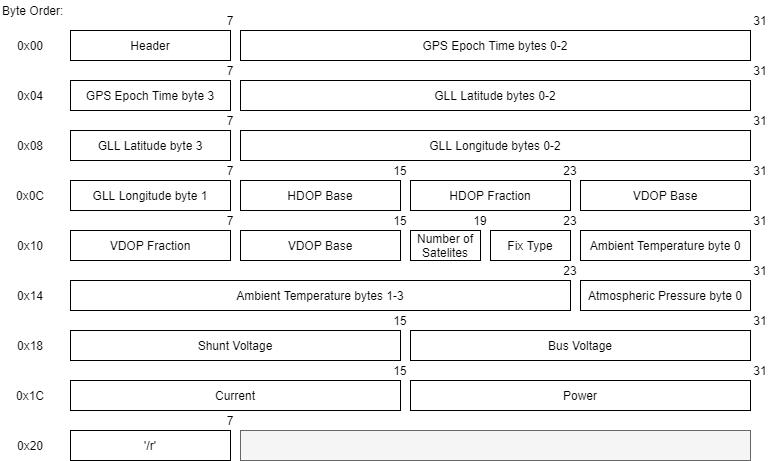
\includegraphics[scale=0.4]{Drift Packet Diagram.png}
    \caption{Diagram showing the structure of a drift data packet including byte position, size and data being collected}
    \label{fig:packet_structure}
\end{figure}

Each Packet begins with a Header. This is an 8-bit value to give information about the data in the payload. This value consist of a 4-bit identifier (0x0 for drift data) as well as a 4-bit number indicating the sample number (1 - 4) before transmission. Data is stored sequentially in little endian format as shown in figure \ref{fig:packet_structure} above. A '\\r' character is used to indicate the end of the packet. This increases the total data requirement from 35 to 37 bytes per sample however, by adding the tail and the header, data integrity is maintained and allow for the standardisation of data transmission.\par  

IMU data however, is of uniform type therefore, no special structures needed to be created. Data from the IMU is stored in an 8-bit buffer array with the most significant byte of the measurement first. Much like the drift buffer, The data was combined into a packet with a header created at the beginning. The header was given the value 0x57 or \textit{"W"} to identify the packet as an IMU data packet. Then the data occupies the remaining bytes with the final byte of the packet assigned to the '<cr>' character to indicate the end of the packet. \par 

Data is stored in the flash chips in packet structure form in the first page of the first available flash chip. Packets are stored sequentially until the device enters transmit state. All data is downloaded from memory and uploaded to the Iridium transmission buffer. The device initiates 2 transmission sessions. First the drift data is uploaded and transmitted, Then the IMU data.Upon successful transmission, the data is sent via satellite network to the Rock7 Rockblock server. The data is saved to a user's account and sent to their email address where the data can be downloaded as an attachment. The diagram below shows the flow of data from the sensors to the user 

\begin{figure}[H]
    \centering
    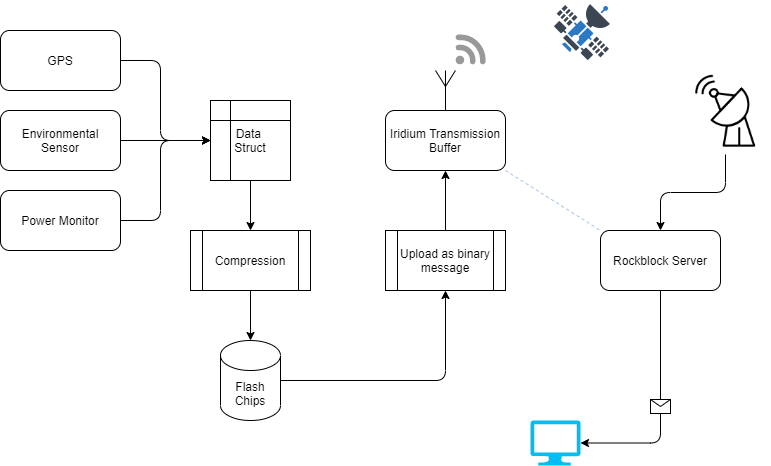
\includegraphics[scale = 0.5]{Data Flow Diagram.png}
    \caption{Diagram showing the flow of data during a cycle of the buoy. The data is sampled by the sensors and converted into packet form where it is stored until it is ready to be transmitted. The transmitted data arrives at a server and is sent via email to the user}
    \label{fig:data_flow}
\end{figure}